\documentclass[11pt,a4paper]{article}
\usepackage{amsmath}
\usepackage{amsfonts}
\usepackage{amssymb}
\usepackage{makeidx}
\usepackage{graphicx}
\usepackage{wrapfig}
\usepackage{enumerate}
\usepackage{pdfpages}
\usepackage{tocloft}
\usepackage{setspace}
\usepackage{mathtools}
\usepackage{hyperref}
\definecolor{linkcolour}{rgb}{0,0.2,0.6} % Link color
\hypersetup{colorlinks,breaklinks,urlcolor=linkcolour,linkcolor=linkcolour}

\usepackage[left=2cm,right=2cm,top=1.5cm,bottom=1.5cm]{geometry}

\usepackage{xcolor}

\usepackage{color,soul}
\usepackage{fontspec}
\setmainfont{Cambria}

\usepackage{caption}
\captionsetup[figure]{font=small, labelfont={bf}}
\captionsetup[table]{font=small, labelfont={bf}}

\usepackage{float}
\usepackage{multirow}
\usepackage{longtable}

\usepackage[nottoc]{tocbibind}

\newcommand{\spa}{\vspace{1.25em}}
\newcommand{\noi}{\noindent}
\def\dul#1{\underline{\underline{#1}}}
\def\cpt#1#2{{\begin{center}\small\textbf{\textcolor{blue}{Figure #1:}} #2\end{center}}}
\def\tt#1{\texttt{#1}}
\def\colortt#1{\textcolor{blue}{\texttt{#1}}}

% for dots in the content
\usepackage{tocloft}
\renewcommand{\cftsecleader}{\cftdotfill{\cftdotsep}}

% For getting paragraphs
\usepackage{titlesec}
\setcounter{secnumdepth}{4}
\setcounter{tocdepth}{4}
\titleformat{\paragraph}
{\normalfont\normalsize\bfseries}{\theparagraph}{1em}{}
\titlespacing*{\paragraph}
{0pt}{3.25ex plus 1ex minus .2ex}{1.5ex plus .2ex}

\begin{document}
	\begin{titlepage} 
		\begin{center}
		\large{ASSIGNMENT 3}\\
		\vspace{2em}
		\large {CS5691 Pattern Recognition and Machine Learning}
		\vspace{3em}
		
		\rule{0.9\linewidth}{0.5mm} \\[0.4cm]
	    {\Large{\bfseries{CS5691 Assignment 3}}} \\
	    \rule{0.9\linewidth}{0.5mm} \\[3 em]	
	    
	    Team Members: \\
	    \vspace{0.5em}
	   	\def\arraystretch{1.25}
\begin{tabular}{c l}
	\hline
	BE17B007 & N Sowmya Manojna \\
	PH17B010 & Thakkar Riya Anandbhai \\
	PH17B011 & Chaithanya Krishna Moorthy \\
	\hline
\end{tabular}

		\vspace{1em}

		Indian Institute of Technology, Madras\\    
		
		\vspace{5em}    
	    
	    	
\includegraphics[scale=0.09]{images/iitmlogo.png}
		\end{center}
	\end{titlepage}

{\hypersetup{linkcolor=black}
 \tableofcontents}
\break


%%%%%%%%%%%%%%%%%%%%%%%%%%%%%%%%%%%%%%%%%%%%%%%
%%%%%%%%%%%%%%%%%%%%%%%%%%%%%%%%%%%%%%%%%%%%%%%
\section{Dataset 1A}
This dataset contains data for four classes - 0, 1, 2 and 3. The classes are linearly separable and the dimension of the feature space is 2.
%%%%%%%%%%%%%%%%%%%%%%%%%%%%%%%%%%%%%%%%%%%%%%%
%%%%%%%%%%%%%%%%%%%%%%%%%%%%%%%%%%%%%%%%%%%%%%%
\subsection{Perceptron}
%%%%%%%%%%%%%%%%%%%%%%%%%%%%%%%%%%%%%%%%%%%%%%%%%%
Varying the hyperparameter : Learning Rate ($\eta$) for the Perceptron model, the accuracies on the training and validation (30\% of the file \colortt{dev.csv}) data for all possible pairings of the classes (leading to a total of 6 pairs ) were obtained and the best $\eta$ value based on CV accuracies was chosen as follows:

%%%%%%%%%%%%%%%%%%%%%%%%%%%%%%%%%%%%%%%%%%%%%%%%%%
\subsubsection{Classes 0 and 1}
%%%%%%%%%%%%%%%%%%%%%%%%%%%%%%%%%%%%%%%%%%%%%%%%%%
\def\arraystretch{1.25}
\begin{center}
{\small
\begin{tabular}{l l l c}
\hline
\hline
\textbf{Hyperparameter}&\textbf{Training Accuracy} & \textbf{CV Accuracy}\\
\hline
\hline
0.001&1.0&1.0\\
0.005&1.0&1.0\\
0.01&1.0&1.0\\
0.05&1.0&1.0\\
0.1&1.0&1.0\\
1.0&1.0&1.0\\
5.0&1.0&1.0\\
10.0&1.0&1.0\\
100.0&1.0&1.0\\
\hline
\end{tabular}

\captionof{table}{Table of training accuracies and CV accuracies for data of classes 0 and 1 of the 1A data set}
}
\end{center}

\noi
The accuracy is 100\% for all values of the hyperparameters. Taking the default value of 0.01, the accuracy on the test data is \textbf{100\%}. The confusion matrices for the training and test data are as in \autoref{fig:perc_conf_01}.
\begin{figure}[H]
    \centering
    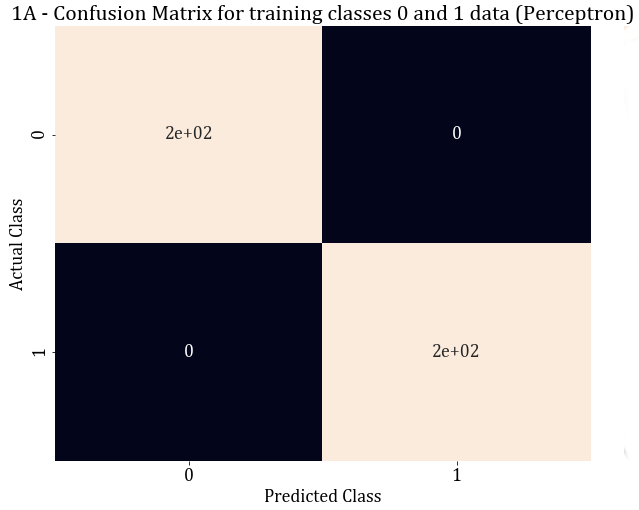
\includegraphics[scale=0.35]{images/1A_perceptron_training_classes_0_and_1_confmat.png}
    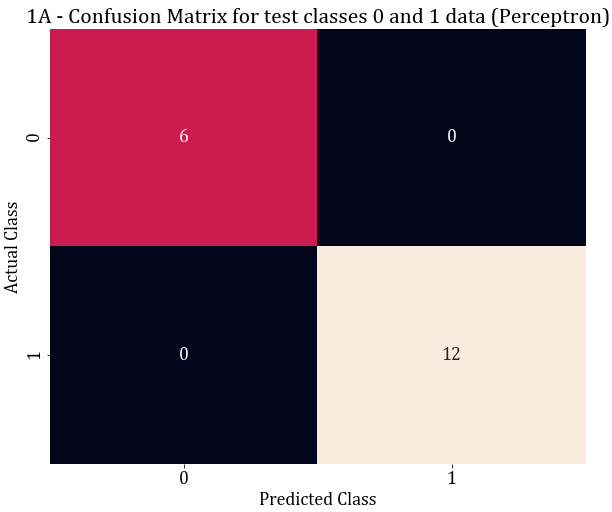
\includegraphics[scale=0.35]{images/1A_perceptron_test_classes_0_and_1_confmat.png}
    \caption{Confusion matrices for training and test data belonging to classes 0 and 1 of data 1A using perceptron classifier}
    \label{fig:perc_conf_01}
\end{figure}

\noi
The decision region plot for the perceptron classifier is in \autoref{fig:perc_dec_reg_01}.
\begin{figure}[H]
    \centering
    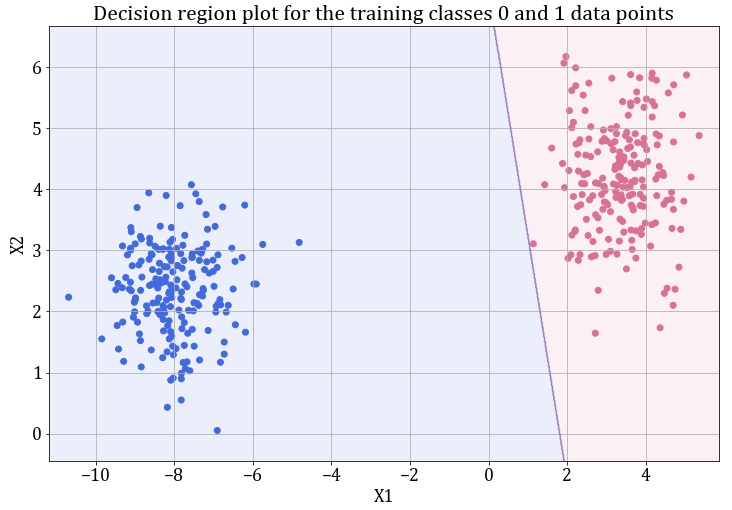
\includegraphics[scale=0.45]{images/1A_perceptron_training_classes_0_and_1_dec_reg.png}
    \caption{Decision region plot for classes 0 and 1 of data 1A using perceptron classifier}
    \label{fig:perc_dec_reg_01}
\end{figure}

%%%%%%%%%%%%%%%%%%%%%%%%%%%%%%%%%%%%%%%%%%%%%%%%%%
\subsubsection{Classes 0 and 2}
%%%%%%%%%%%%%%%%%%%%%%%%%%%%%%%%%%%%%%%%%%%%%%%%%%
\def\arraystretch{1.25}
\begin{table}[H]
{\small
\centering
\begin{tabular}{l l l c}
\hline
\hline
\textbf{Hyperparameter} & \textbf{Training Accuracy}  &  \textbf{CV Accuracy}\\
\hline
\hline
0.001 & 100.0 & 100.0\\
0.005 & 100.0 & 100.0\\
0.01 & 100.0 & 100.0\\
0.05 & 100.0 & 100.0\\
0.1 & 100.0 & 100.0\\
1.0 & 100.0 & 100.0\\
5.0 & 100.0 & 100.0\\
10.0 & 100.0 & 100.0\\
100.0 & 100.0 & 100.0\\
\hline
\end{tabular}
\caption{Training and CV accuracies for classes 0 and 2 of dataset 1A.}
}
\end{table}

\noi
The accuracy is 100\% for all values of the hyperparameters. Taking the default value of 0.01, the accuracy on the test data is \textbf{100\%}. The confusion matrices for the training and test data are as in \autoref{fig:perc_conf_02}.
\begin{figure}[H]
    \centering
    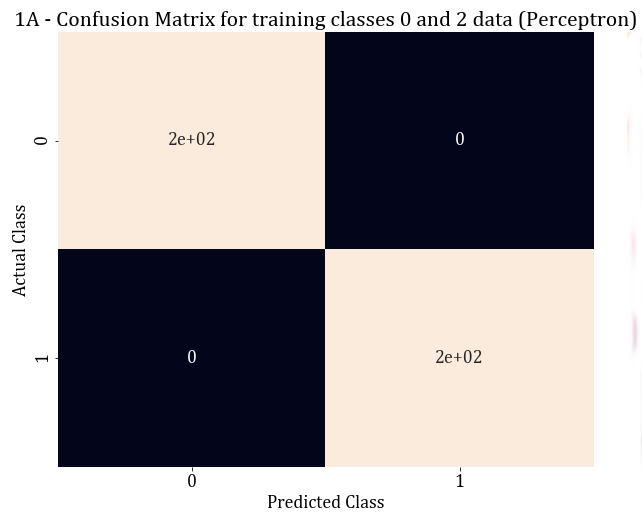
\includegraphics[scale=0.35]{images/1A_perceptron_training_classes_0_and_2_confmat.png}
    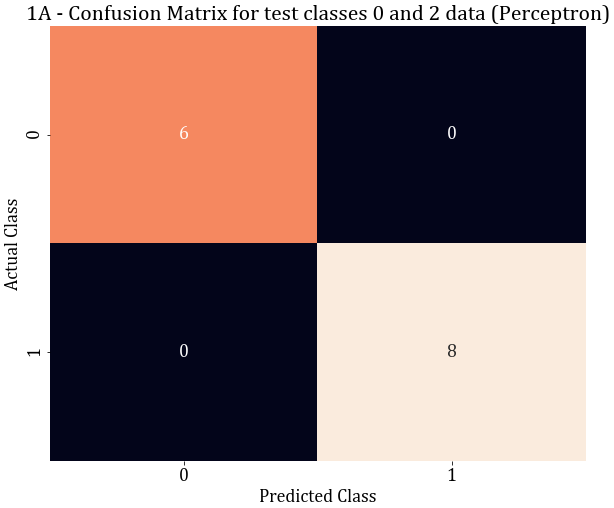
\includegraphics[scale=0.35]{images/1A_perceptron_test_classes_0_and_2_confmat.png}
    \caption{Confusion matrices for training and test data belonging to classes 0 and 2 of data 1A using perceptron classifier}
    \label{fig:perc_conf_02}
\end{figure}

\noi
The decision region plot for the perceptron classifier is in \autoref{fig:perc_dec_reg_02}.
\begin{figure}[H]
    \centering
    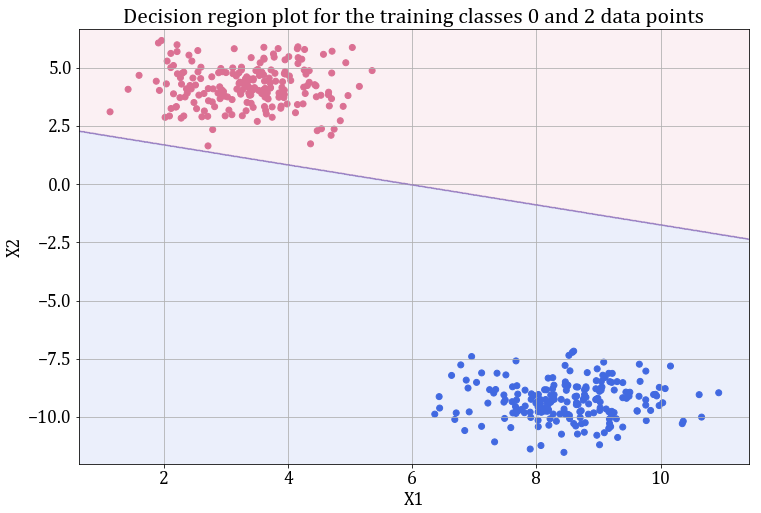
\includegraphics[scale=0.45]{images/1A_perceptron_training_classes_0_and_2_dec_reg.png}
    \caption{Decision region plot for classes 0 and 2 of data 1A using perceptron classifier}
    \label{fig:perc_dec_reg_02}
\end{figure}

%%%%%%%%%%%%%%%%%%%%%%%%%%%%%%%%%%%%%%%%%%%%%%%%%%
\subsubsection{Classes 0 and 3}
%%%%%%%%%%%%%%%%%%%%%%%%%%%%%%%%%%%%%%%%%%%%%%%%%%
\def\arraystretch{1.25}
\begin{center}
{\small
\begin{tabular}{l l l c}
\hline
\hline
\textbf{Hyperparameter}&\textbf{Training Accuracy} & \textbf{CV Accuracy}\\
\hline
\hline
0.001&1.0&1.0\\
0.005&1.0&1.0\\
0.01&1.0&1.0\\
0.05&1.0&1.0\\
0.1&1.0&1.0\\
1.0&1.0&1.0\\
5.0&1.0&1.0\\
10.0&1.0&1.0\\
100.0&1.0&1.0\\
\hline

\end{tabular}

\captionof{table}{Table of training accuracies and CV accuracies for data of classes 0 and 3 of the 1A data set}
}
\end{center}

The accuracy is 100\% for all values of the hyperparameters. Taking the default value of 0.01, the accuracy on the test data is \textbf{100\%}. The confusion matrices for the training and test data are as in \autoref{fig:perc_conf_03}.
\begin{figure}[H]
    \centering
    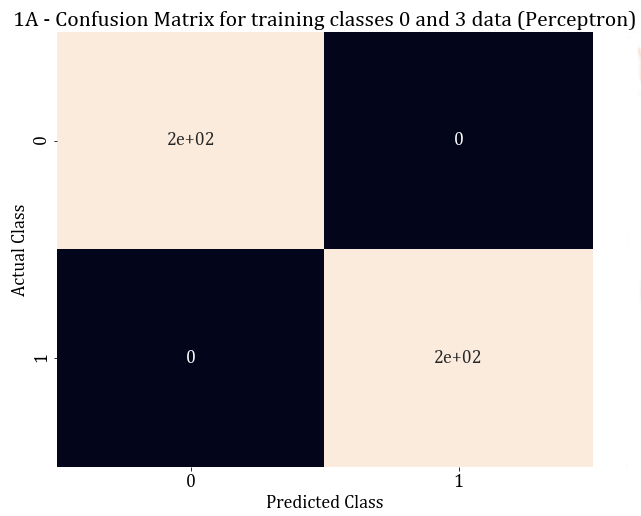
\includegraphics[scale=0.3]{images/1A_perceptron_training_classes_0_and_3_confmat.png}
    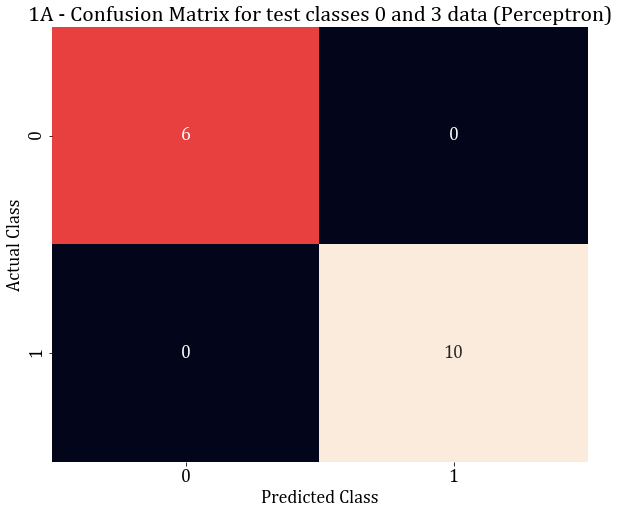
\includegraphics[scale=0.3]{images/1A_perceptron_test_classes_0_and_3_confmat.png}
    \caption{Confusion matrices for training and test data belonging to classes 0 and 3 of data 1A using perceptron classifier}
    \label{fig:perc_conf_03}
\end{figure}
The decision region plot for the perceptron classifier is in \autoref{fig:perc_dec_reg_03}.
\begin{figure}[H]
    \centering
    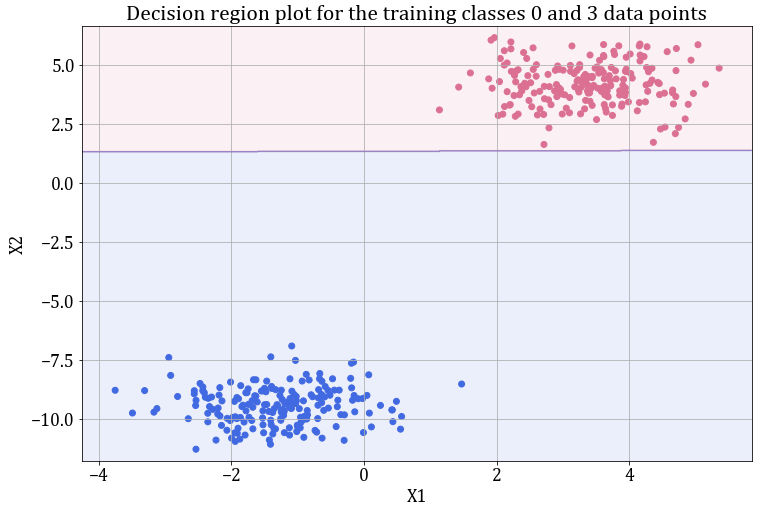
\includegraphics[scale=0.45]{images/1A_perceptron_training_classes_0_and_3_dec_reg.png}
    \caption{Decision region plot for classes 0 and 3 of data 1A using perceptron classifier}
    \label{fig:perc_dec_reg_03}
\end{figure}

%%%%%%%%%%%%%%%%%%%%%%%%%%%%%%%%%%%%%%%%%%%%%%%%%%
\subsubsection{Classes 1 and 2}
%%%%%%%%%%%%%%%%%%%%%%%%%%%%%%%%%%%%%%%%%%%%%%%%%%
\def\arraystretch{1.25}
\begin{center}
{\small
\begin{tabular}{l l l c}
\hline
\hline
\textbf{Hyperparameter}&\textbf{Training Accuracy} & \textbf{CV Accuracy}\\
\hline
\hline
0.001&1.0&0.975\\
0.005&1.0&0.975\\
0.01&1.0&0.975\\
0.05&1.0&1.0\\
0.1&1.0&1.0\\
1.0&1.0&1.0\\
5.0&1.0&1.0\\
10.0&1.0&1.0\\
100.0&1.0&1.0\\
\hline
\end{tabular}

\captionof{table}{Table of training accuracies and CV accuracies for data of classes 1 and 2 of the 1A data set}
}
\end{center}

The accuracy on the CV data is best for $\eta = 0.05$. Using this value for the perceptron model, the accuracy on the test data is \textbf{100\%}. The confusion matrices for the training and test data are as in \autoref{fig:perc_conf_12}.

\begin{figure}[H]
    \centering
    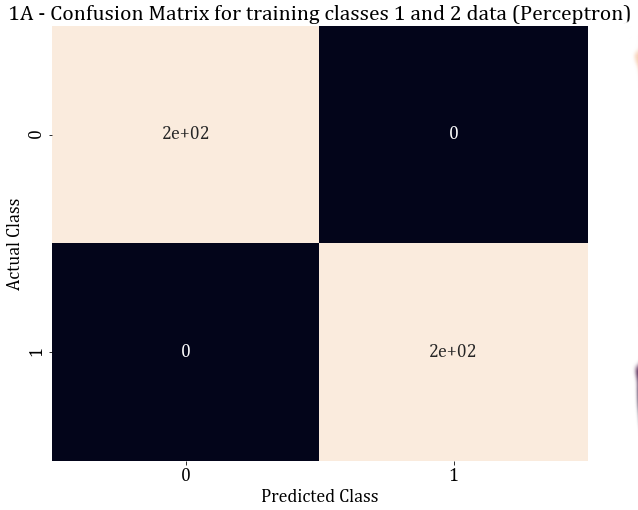
\includegraphics[scale=0.3]{images/1A_perceptron_training_classes_1_and_2_confmat.png}
    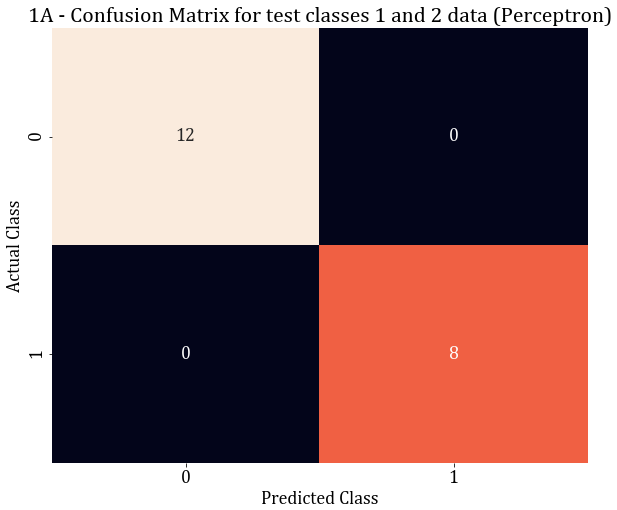
\includegraphics[scale=0.3]{images/1A_perceptron_test_classes_1_and_2_confmat.png}
    \caption{Confusion matrices for training and test data belonging to classes 1 and 2 of data 1A using perceptron classifier}
    \label{fig:perc_conf_12}
\end{figure}
The decision region plot for the perceptron classifier is in \autoref{fig:perc_dec_reg_12}.
\begin{figure}[H]
    \centering
    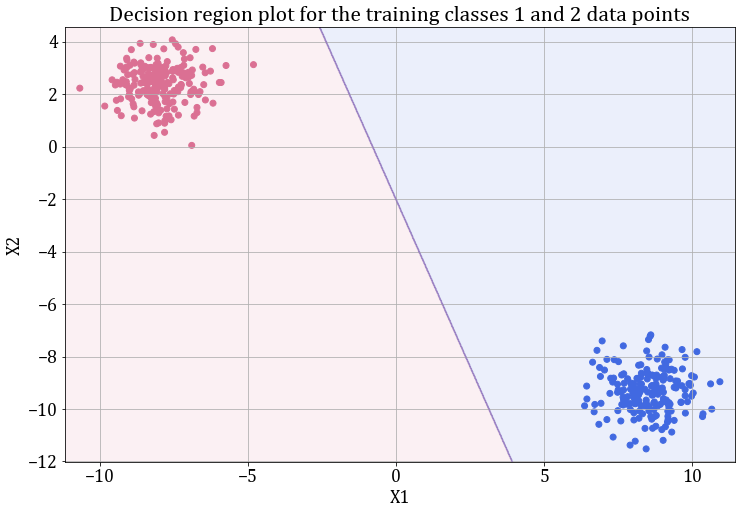
\includegraphics[scale=0.45]{images/1A_perceptron_training_classes_1_and_2_dec_reg.png}
    \caption{Decision region plot for classes 1 and 2 of data 1A using perceptron classifier}
    \label{fig:perc_dec_reg_12}
\end{figure}

%%%%%%%%%%%%%%%%%%%%%%%%%%%%%%%%%%%%%%%%%%%%%%%
\subsubsection{Classes 1 and 3}
%%%%%%%%%%%%%%%%%%%%%%%%%%%%%%%%%%%%%%%%%%%%%%%%%%
\def\arraystretch{1.25}
\begin{table}[H]
{\small
\centering
\begin{tabular}{l l l l l l}
\hline
\hline
\textbf{Hyperparameter}&\textbf{Training Accuracy} & \textbf{CV Accuracy} & \textbf{Hyperparameter}&\textbf{Training Accuracy} & \textbf{CV Accuracy}\\
\hline
\hline
0.001 & 100.0 & 100.0 & 1.0 & 100.0 & 100.0\\
0.005 & 100.0 & 100.0 & 5.0 & 100.0 & 100.0\\
0.01 & 100.0 & 100.0 & 10.0 & 100.0 & 100.0\\
0.05 & 100.0 & 100.0 & 100.0 & 100.0 & 100.0\\
0.1 & 100.0 &100.0 & & & \\
\hline
\end{tabular}
\caption{Training and CV accuracies for classes 1 and 3 of dataset 1A.}
}
\end{table}
The accuracy is 100\% for all values of the hyperparameters. Taking the default value of 0.01, the accuracy on the test data is \textbf{100\%}. The confusion matrices for the training and test data are as in \autoref{fig:perc_conf_13}.
\begin{figure}[H]
    \centering
    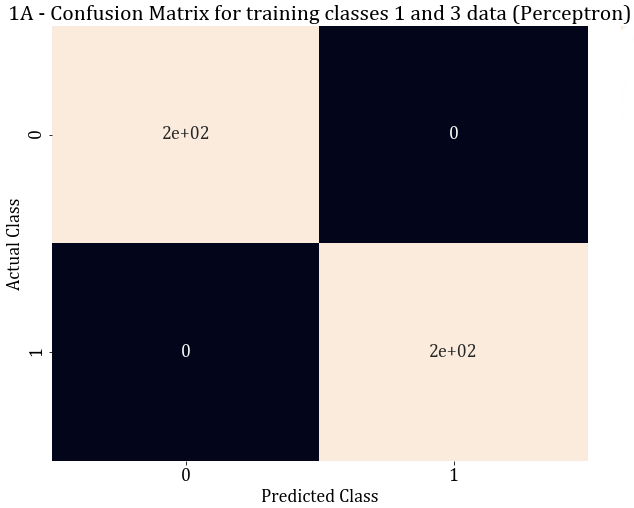
\includegraphics[scale=0.35]{images/1A_perceptron_training_classes_1_and_3_confmat.png}
    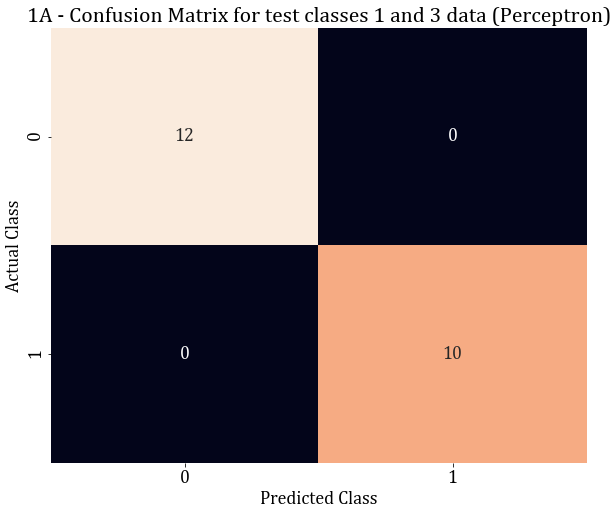
\includegraphics[scale=0.35]{images/1A_perceptron_test_classes_1_and_3_confmat.png}
    \caption{Confusion matrices for training and test data belonging to classes 1 and 3 of data 1A using perceptron classifier}
    \label{fig:perc_conf_13}
\end{figure}

\noi
The decision region plot for the perceptron classifier is in \autoref{fig:perc_dec_reg_13}.
\begin{figure}[H]
    \centering
    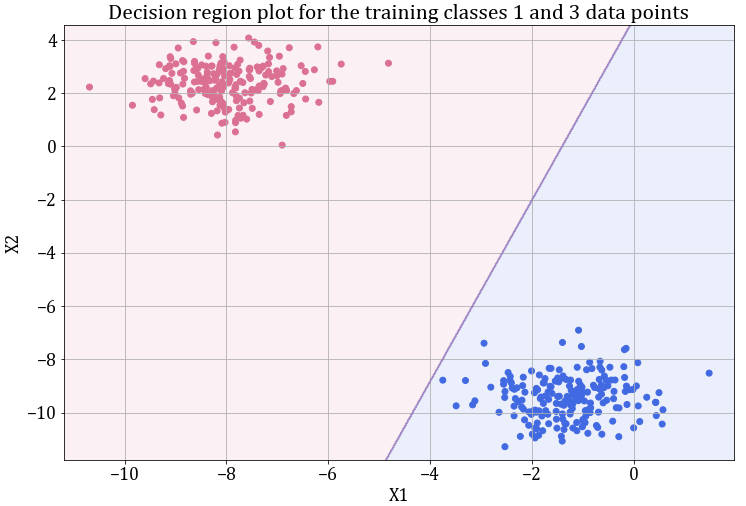
\includegraphics[scale = 0.45]{images/1A_perceptron_training_classes_1_and_3_dec_reg.png}
    \caption{Decision region plot for classes 1 and 3 of data 1A using perceptron classifier}
    \label{fig:perc_dec_reg_13}
\end{figure}


%%%%%%%%%%%%%%%%%%%%%%%%%%%%%%%%%%%%%%%%%%%%%%%
\subsubsection{Classes 2 and 3}
%%%%%%%%%%%%%%%%%%%%%%%%%%%%%%%%%%%%%%%%%%%%%%%%%%
\def\arraystretch{1.25}
\begin{table}[H]
{\small
\centering
\begin{tabular}{l l l l l l}
\hline
\hline
\textbf{Hyperparameter}&\textbf{Training Accuracy} & \textbf{CV Accuracy} & \textbf{Hyperparameter}&\textbf{Training Accuracy} & \textbf{CV Accuracy}\\
\hline
\hline
0.001 & 100.0 & 92.86 & 1.0 & 100.0 & 100.0\\
0.005 & 100.0 & 100.0 & 5.0 & 100.0 & 97.62\\
0.01 & 100.0 & 100.0 & 10.0 & 100.0 & 100.0\\
0.05 & 100.0 & 100.0 & 100.0 & 100.0 & 100.0\\
0.1 & 100.0 & 100.0 & & & \\
\hline
\end{tabular}
\caption{Training and CV accuracies for classes 2 and 3 of dataset 1A.}
}
\end{table}
The accuracy on the CV data is best for $\eta$ greater than or equal to 0.005. Using the default value of $\eta = 0.01$ for the perceptron model, the accuracy on the test data is \textbf{100\%}. The confusion matrices for the training and test data are as in \autoref{fig:perc_conf_23}.
\begin{figure}[H]
    \centering
    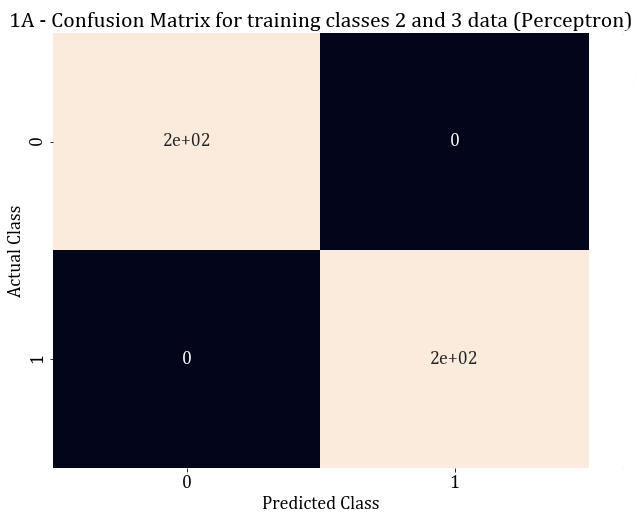
\includegraphics[scale=0.35]{images/1A_perceptron_training_classes_2_and_3_confmat.png}
    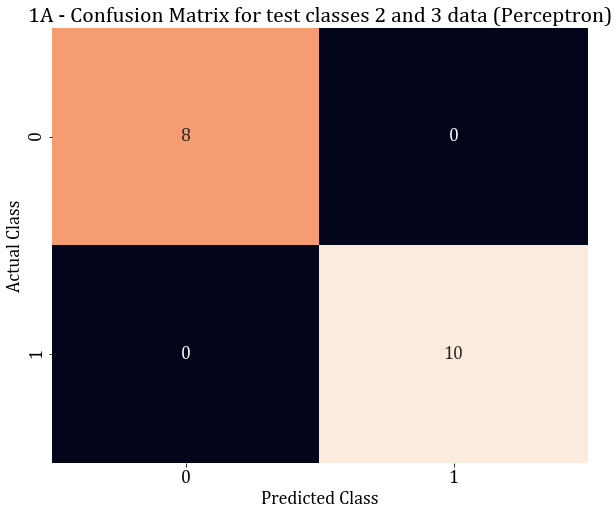
\includegraphics[scale=0.35]{images/1A_perceptron_test_classes_2_and_3_confmat.png}
    \caption{Confusion matrices for training and test data belonging to classes 2 and 3 of data 1A using perceptron classifier}
    \label{fig:perc_conf_23}
\end{figure}

\noi
The decision region plot for the perceptron classifier is in \autoref{fig:perc_dec_reg_23}.
\begin{figure}[H]
    \centering
    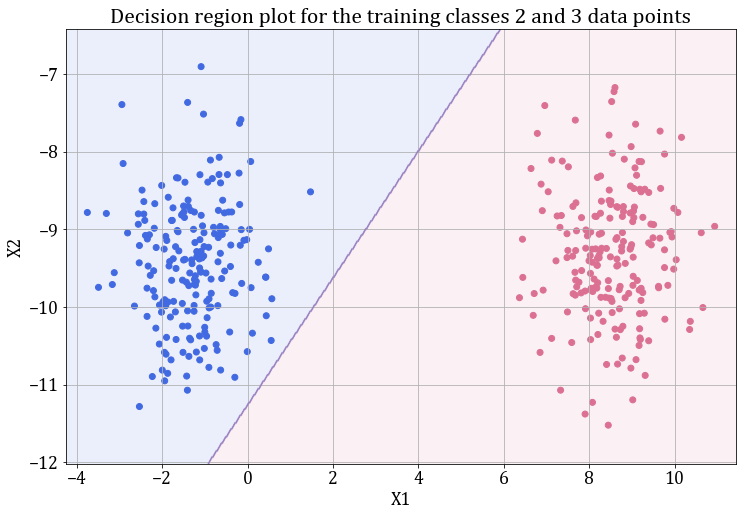
\includegraphics[scale = 0.45]{images/1A_perceptron_training_classes_2_and_3_dec_reg.png}
    \caption{Decision region plot for classes 2 and 3 of data 1A using perceptron classifier}
    \label{fig:perc_dec_reg_23}
\end{figure}

%%%%%%%%%%%%%%%%%%%%%%%%%%%%%%%%%%%%%%%%%%%%%%%
\subsection{MLFFNN}
%%%%%%%%%%%%%%%%%%%%%%%%%%%%%%%%%%%%%%%%%%%%%%%%%%
The hyperparameters varied and sweeped for are - \tt{hidden layer size}, \tt{optimizer}, \tt{batch size}, \tt{learning rate}, \tt{L2 regularization $\alpha$}. They were varied as follows:
\begin{itemize}
    \itemsep0em
    \item \tt{hidden\_layer\_sizes}: 5,8,10,15
    \item \tt{activation}: \tt{logistic}, \tt{tanh}, \tt{relu}
    \item \tt{solver}: \tt{lbfgs}, \tt{sgd}, \tt{adam}
    \item \tt{batch\_size}: 100, 200
    \item \tt{alpha}: 0, 0.0001
    \item \tt{learning\_rate}: \tt{constant}, \tt{adaptive}, \tt{invscaling}
\end{itemize}

\noi
Hence, a total of 432 parameter combinations were sweeped for and analyzed.

\subsubsection{Classification Accuracies}
The classification accuracies on the training and validation datasets (30\% of the \colortt{dev.csv}) are as follows:
\def\arraystretch{1.25}
\begin{center}
{\small
\begin{tabular}{l l l l l l l c}
\hline
\hline
\textbf{\# Neurons} & \textbf{Activation} & \textbf{Solver} & \textbf{Batch Size} & \textbf{\alpha} & \textbf{Learning Rate} & \textbf{Accuracy} & \textbf{Validation Accuracy} \\
\hline
\hline
5 & tanh & lbfgs & 200 & 0.0001 & adaptive & 100.0 & 100.0 \\
5 & tanh & lbfgs & 200 & 0.0001 & constant & 100.0 & 100.0 \\
5 & tanh & lbfgs & 200 & 0.0 & invscaling & 100.0 & 100.0 \\
5 & tanh & lbfgs & 200 & 0.0 & adaptive & 100.0 & 100.0 \\
5 & tanh & lbfgs & 200 & 0.0 & constant & 100.0 & 100.0 \\
5 & tanh & lbfgs & 100 & 0.0 & adaptive & 100.0 & 100.0 \\
5 & tanh & lbfgs & 100 & 0.0001 & invscaling & 100.0 & 100.0 \\
5 & relu & lbfgs & 200 & 0.0 & constant & 100.0 & 100.0 \\
5 & relu & lbfgs & 100 & 0.0001 & invscaling & 100.0 & 100.0 \\
5 & relu & lbfgs & 200 & 0.0 & adaptive & 100.0 & 100.0 \\
\hline
\end{tabular}
\setcounter{table}{1}
\captionof{table}{Best 10 Train and Validation Accuracies obtained after performing a \colortt{GridSearch} on 432 parameter combinations.}
}
\end{center}

\subsubsection{Best Model}
The parameter combination were additionally sorted based on minimum fitting time (least fitting time - first) and the model that gave the best accuracy the fastest (and potentially the most minimal model that best fits the data), was chosen. Hence the best parameter combination chosen is:
\begin{itemize}
    \itemsep0em
    \item \tt{hidden\_layer\_sizes}: 5
    \item \tt{activation}: tanh
    \item \tt{solver}: lbfgs
    \item \tt{batch\_size}: 200
    \item \tt{alpha}: 0.0001
    \item \tt{learning\_rate}: adaptive
\end{itemize}

\noi
The classification accuracy of the best model on the testing data is: \textbf{100\%}. The confusion matrices obtained are as follows:
\begin{figure}[H]
    \centering
    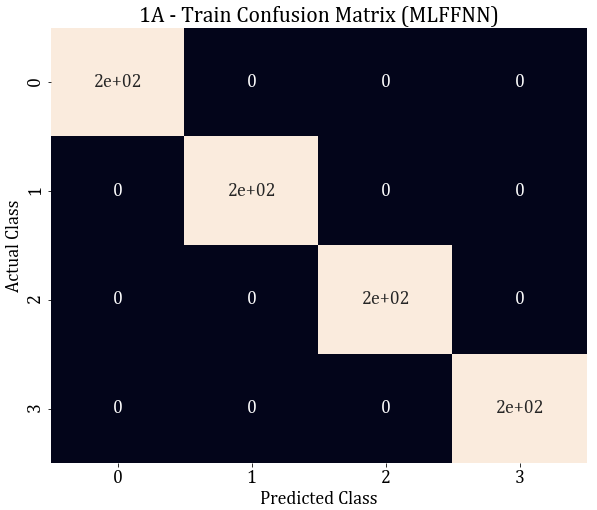
\includegraphics[scale=0.4]{images/1A_MLFFNN_train_confmat.png}
    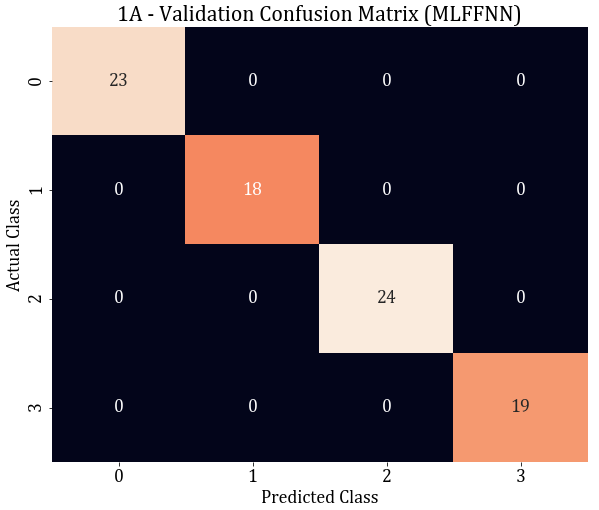
\includegraphics[scale=0.4]{images/1A_MLFFNN_val_confmat.png}
    \caption{Training and Validation confusion matrices obtained for the best parameter combination, on the left and right respectively.}
\end{figure}

\begin{figure}[H]
    \centering
    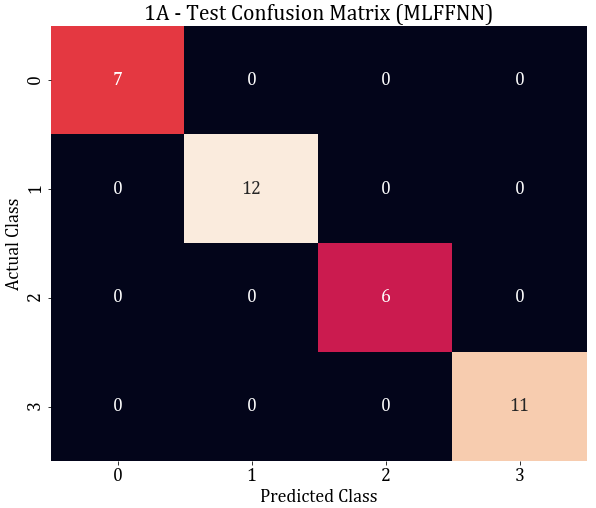
\includegraphics[scale=0.45]{images/1A_MLFFNN_test_confmat.png}
    \caption{Testing confusion matrices obtained for the best parameter combination.}
\end{figure}

\subsubsection{Decision Region}
The decision region plots obtained is as follows:
\begin{figure}[H]
    \centering
    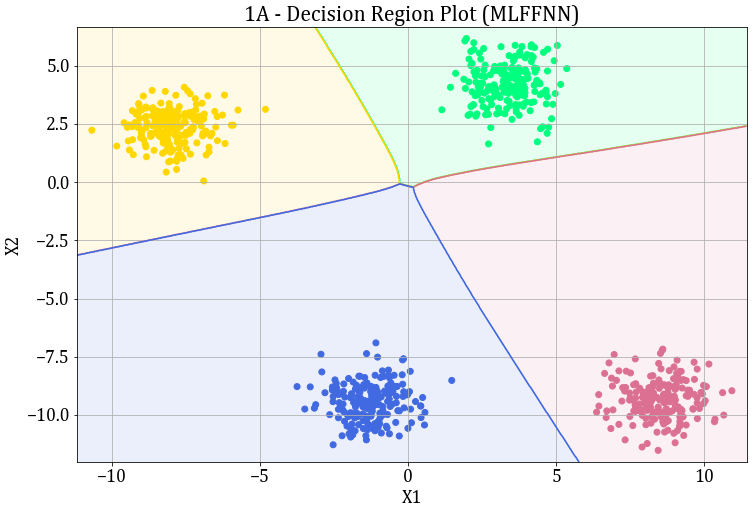
\includegraphics[scale=0.6]{images/1A_MLFFNN_Decision_Plot.png}
    \caption{Decision Region Plot obtained for the best parameter combination.}
\end{figure}

%%%%%%%%%%%%%%%%%%%%%%%%%%%%%%%%%%%%%%%%%%%%%%%
\subsection{Linear SVM}
%%%%%%%%%%%%%%%%%%%%%%%%%%%%%%%%%%%%%%%%%%%%%%%%%%

\label{subsection:1A_svm}
The Support Vector Machines (SVMs) are supervised learning models that can be used for regression, classification and outlier detection. In case of a linear classifier, the goal of the SVM is to construct a hyperplane(s) such that the distance from the nearest training data point is maximized. This distance is called the functional margin.  


\subsubsection{Mathematical Formulation}
\noindent
For a hyperplane of the form:
\begin{equation}
    g(\vec{x})=\vec{w^{T}}*\vec{x}-w_{0}=0
\end{equation}
\noi
The distance of any point $\vec{x}$ from the hyperplane is then equivalent to: 
\begin{equation}
    r=\frac{g(\vec{x})}{||w||}
\end{equation}
\noi
For a canonically seperating hyperplane, 
\begin{equation}
    |g_c(\vec{x^*})|=1
\end{equation}
\noi
Where $\vec{x^*}$ is the training example nearest to the hyperplane. 
The distance of $\vec{x^*}$ from the hyperplane is then given by:
\begin{equation}
    r=\frac{1}{||\vec{w}||}
\end{equation}
\noi
For all points $(\vec{x_n},t_n)$, 
\begin{equation}
    (t_n)(\vec{w}^{T}X_n+w_0) \geq 1
\end{equation}
\noi
Where $t_n$ is the target variable $\epsilon$ $(-1,1)$.
\noi
The primal form of the Lagrangian objective function is:
\begin{equation}
    L_p(\vec{w},w_0,\vec{\alpha})=\frac{||\vec{w}||}{2}-\sum_{n=1}^{N}\alpha_n[t_n(\vec{w}^T\vec{x_n}+w_0)-1]
\end{equation}

\noi
Optimality condition:
\begin{equation}
    \frac{\partial L_p}{\partial \vec{w}}=\vec{0}
\end{equation}

\begin{equation}
    \frac{\partial L_p}{\partial w_0}=0
\end{equation}

\noi
Substituting the form of $L_p$ and differentiating:
\begin{equation}
    \vec{w}-\sum_{n=1}^{N}\alpha_nt_n\vec{x_n}=\vec{0}
\end{equation}

\begin{equation}
    \sum_{n=1}^{N}\alpha_nt_n=0
\end{equation}

\noi
The dual form of Lagrangian can be obtained by substituting the form of $\vec{w}$ in the primal form.\\ 
The task is now to find $\vec{\alpha}$ for which $L_D(\vec{\alpha)}$ is optimal subject to $\alpha_n\geq 0$. This is a quadratic problem and can be solved by a QP solver.
\begin{equation}
    L_D(\vec{\alpha})=\sum_{n=1}^{N}\alpha_n-\frac{1}{2}\sum_{m=1}^{N}\sum_{n=1}^{N}\alpha_m\alpha_nt_mt_n\vec{x_m}^T\vec{x_n} 
\end{equation}

\subsubsection{svm.SVC() function in the scikit-learn library}\label{subsubsection:svm module}
The svm.SVC() is a pre-defined module for Support Vector Classification task. The important optional arguments of this classifier are: 
\begin{itemize}
    \item \tt{kernel} : Specifies the kernel type to be used in the algorithm, available options are: [\tt{linear},\tt{poly},\tt{rbf},\tt{sigmoid},\tt{precomputed}].
    The default kernel is the rbf(/gaussian). 
    \begin{itemize}
        \item Linear kernel: $<x,x'>$
        \item Polynomial kernel: $(\gamma<x,x'>+r)^{d}$
        \item RBF kernel: $-\gamma||x-x'||^{2}$
        \item sigmoid kernel: tanh$(\gamma<x,x'>+r)$
    \end{itemize} 

    \noi
    For dataset 1A, linear kernel is used. 
    \item \tt{C}: strictly positive float. By default it is 1.0. The strength of regularization is inversely proportional to C. For dataset 1A, C is varied from 0.1 to 1000. 
    \item \tt{degree}: This is relevant only when the kernel is set to polynomial and is ignored by all other kernel values.
    \item \tt{gamma}: float or [\tt{scale}, \tt{auto}]. Set to \tt{scale} by default, it is the kernel coefficient for \tt{rbf}, \tt{poly} and \tt{sigmoid}.
    \item \tt{decision\_function\_shape}: [\tt{ovr}, \tt{ovo}]. It specifies whether one-versus-rest or one-versus-one methodology should be used for multi-class classification. By default, it is \tt{ovr}. 
\end{itemize}

\subsubsection{Building pairwise SVM for classes in dataset 1A}
The dataset 1A has 4 class labels: [0.0,1.0,2.0,3.0], and 2 dimensional feature vectors. Those are linearly separable as can be seen in the plot above.
\begin{itemize}
    \item Data pre-processing:
    \begin{itemize}
        \item There are no missing values in the data.
        \item The ranges of feature vectors are nearly same, hence scaling is not essential. 
    \end{itemize}
    \item The data is then split according to the class labels to further build one-vs-one svm models.
    \item sklearn.svm.SVC(),with a linear kernel is then trained using a pair of classes at once, hence, number of models trained is $\frac{3(3+1)}{2}=6$. 
    \item The decision boundary and support vectors are then obtained for each of those models. However, the decision region for y[i] vs y[j] model is defined only for x1 and x2 range where y[i] and y[j] exist in the training data
    \item To predict the class label for a test point: we obtain 6 labels from the 6 different models trained earlier. From those 6 labels, the label occurring with the most frequency is chosen as the label for the test point, a collective decision region and confusion matrix are thus obtained.
\end{itemize}

\subsubsection{Hyper-parameter value and accuracy}
The hyper-parameter C is varied in the range [0.1,1,10,100,1000] and corresponding accuracy over train data and cross validation data is obtained as follows: 

\def\arraystretch{1.25}
\begin{table}[H]
\centering
\begin{tabular}{l l l }
\hline
\hline
\textbf{C} & \textbf{Train accuracy} & \textbf{Validation Accuracy} \\
\hline
\hline
0.1 & 1.00 & 1.00\\
1 & 1.00 & 1.00\\
10 & 1.00 & 1.00\\
100 & 1.00 & 1.00\\
1000 & 1.00 & 1.00\\
\hline
\end{tabular}
\caption{Accuracy table for dataset 1A, Pairwise Linear SVM}
\end{table}
\noi
Since the accuracy is independent of the value of hyper-parameter C, the default value C=1 is used for the production of plots and confusion matrices.The accuracy obtained on test data set is also 1.00 

\noi
\subsubsection{Confusion matrices for Train and Test data}
Since the accuracy obtained is 1.00, the confusion matrices are diagonal. 
\begin{figure}[H]
\centering
    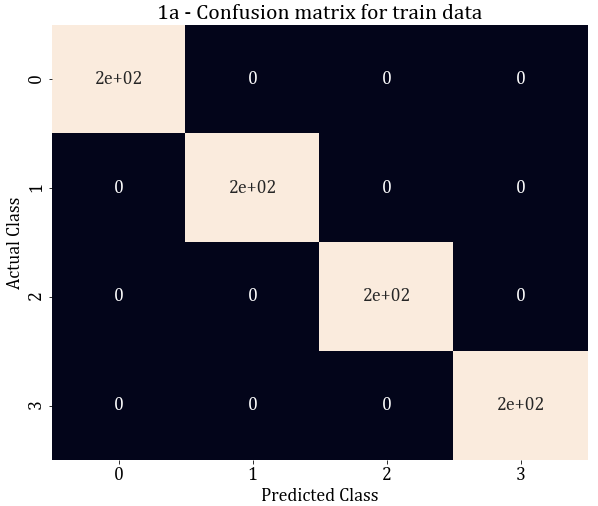
\includegraphics[scale=0.4]{images/1A_confmatrix_train.png}
    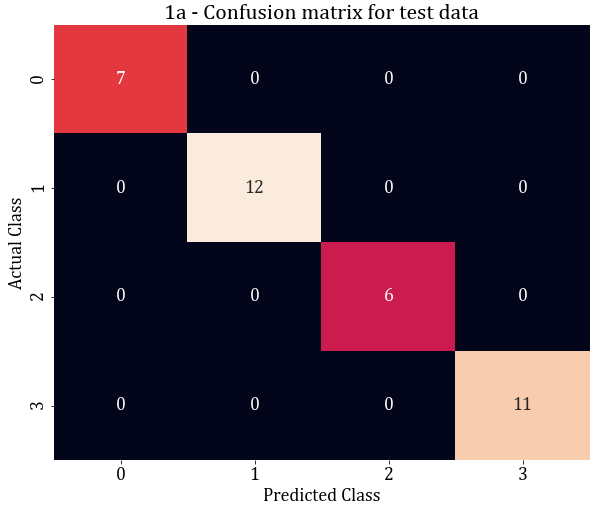
\includegraphics[scale=0.4]{images/1A_confmatrix_test.png}
    \caption{Confusion matrix for train and test data respectively}
\end{figure}

\begin{figure}[H]
\centering
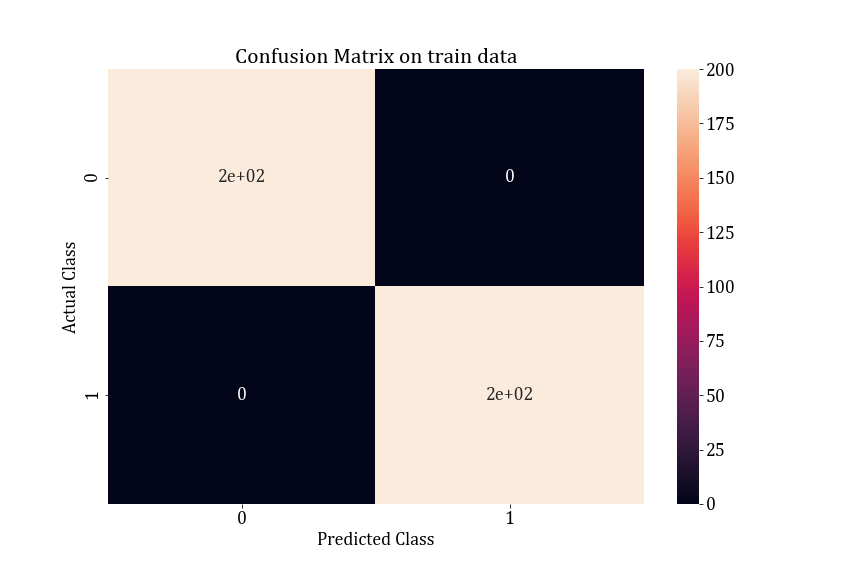
\includegraphics[scale=0.4]{images/1A_ovo_conf01_train.png}
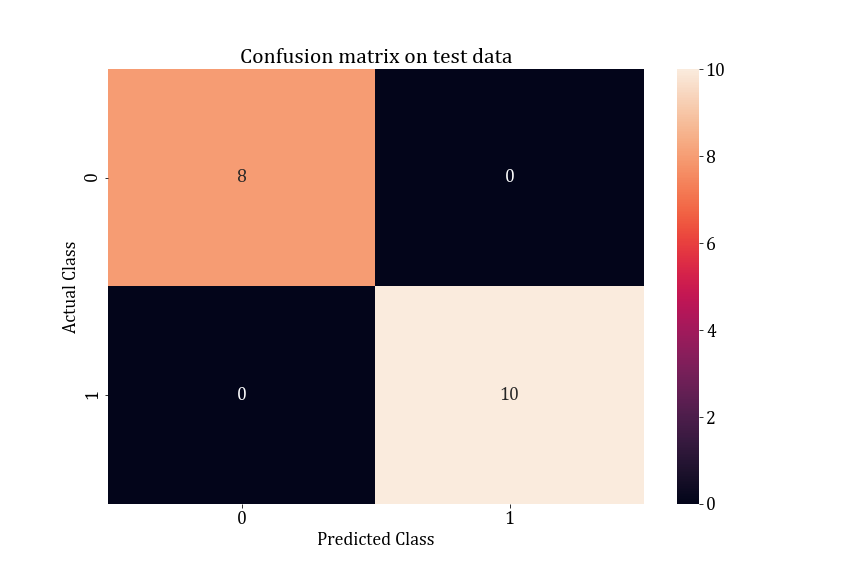
\includegraphics[scale=0.4]{images/1A_ovo_conf01_test.png}
\caption{Confusion matrix for class 0 and 1, train and test data respectively}
\end{figure}

\begin{figure}[H]
\centering
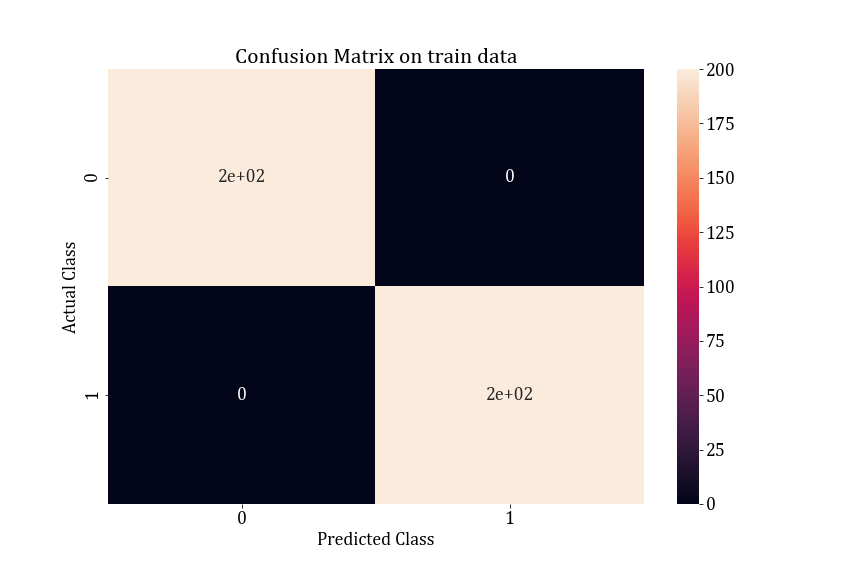
\includegraphics[scale=0.4]{images/1A_ovo_conf02_train.png}
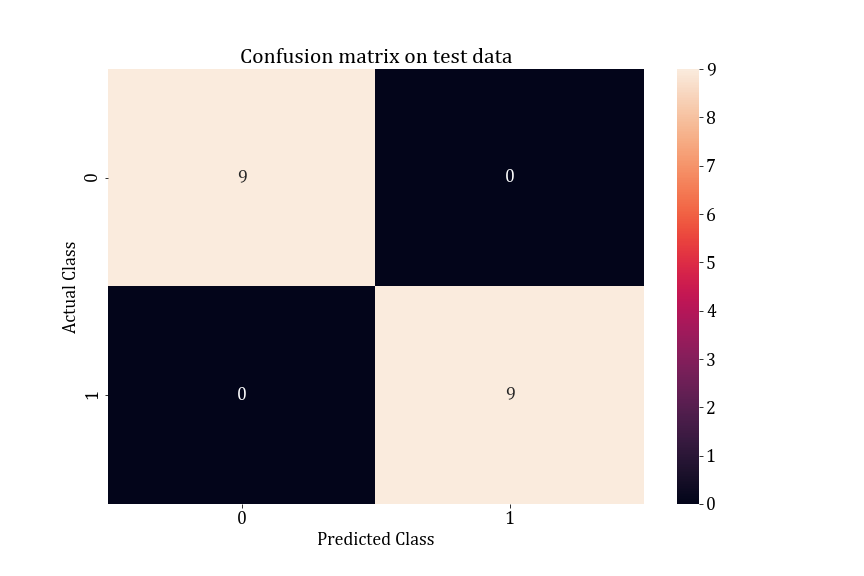
\includegraphics[scale=0.4]{images/1A_ovo_conf02_test.png}
\caption{Confusion matrix for class 0 and 2, train and test data respectively}
\end{figure}

\begin{figure}[H]
\centering
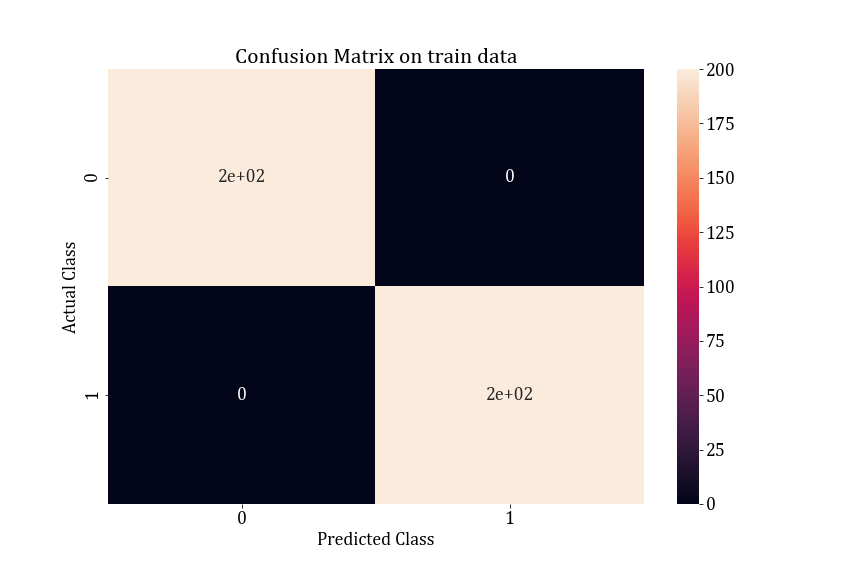
\includegraphics[scale=0.4]{images/1A_ovo_conf03_train.png}
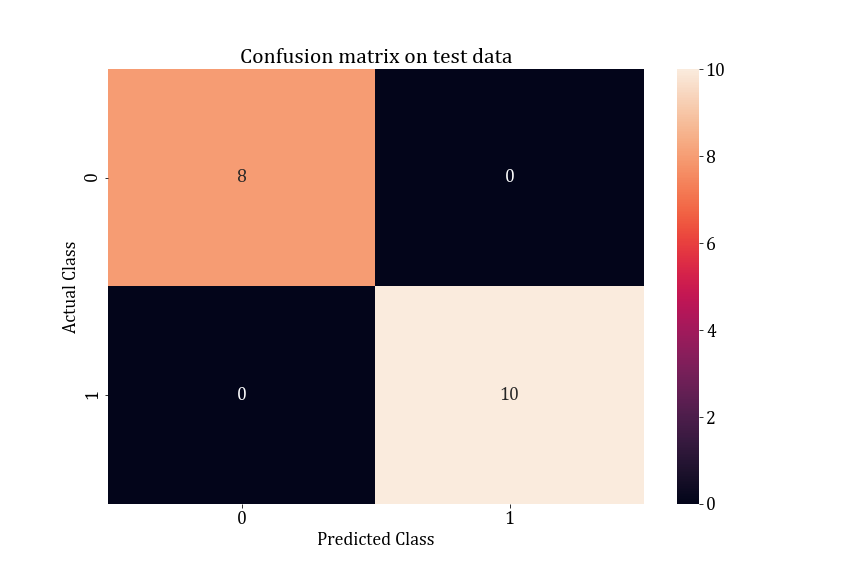
\includegraphics[scale=0.4]{images/1A_ovo_conf03_test.png}
\caption{Confusion matrix for class 0 and 3, train and test data respectively}
\end{figure}

\begin{figure}[H]
\centering
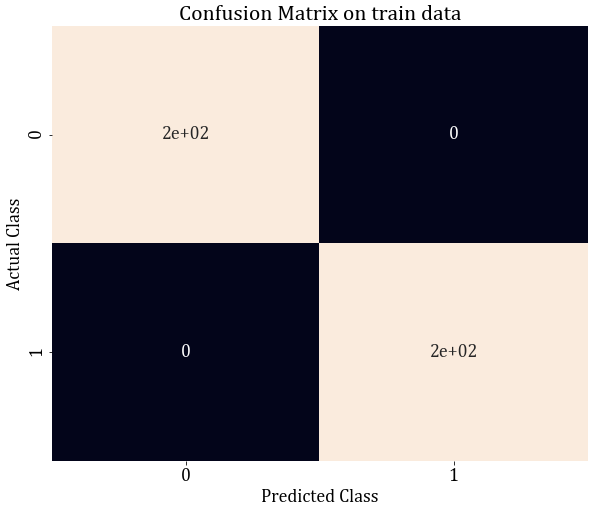
\includegraphics[scale=0.4]{images/1A_ovo_conf12_train.png}
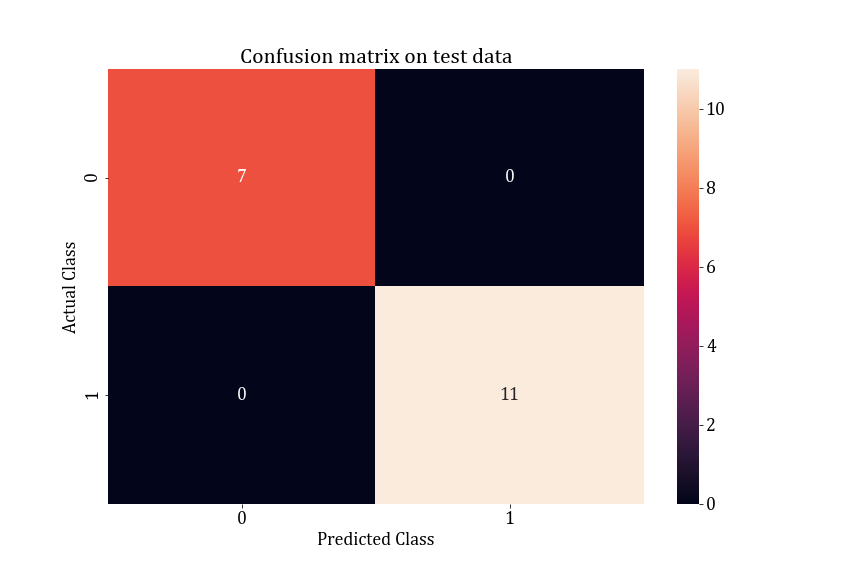
\includegraphics[scale=0.4]{images/1A_ovo_conf12_test.png}
\caption{Confusion matrix for class 1 and 2, train and test data respectively}
\end{figure}

\begin{figure}[H]
\centering
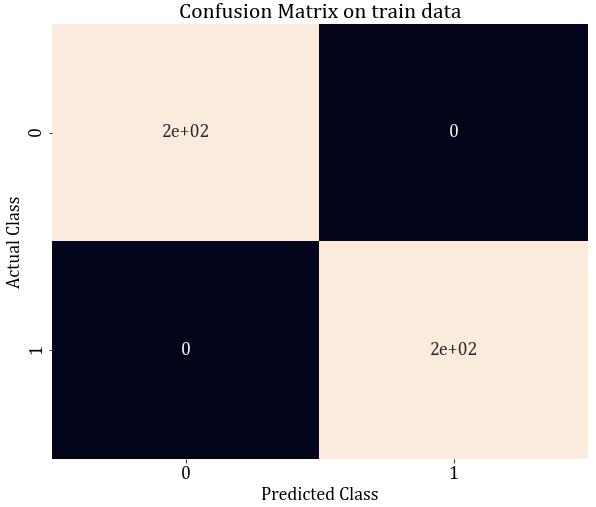
\includegraphics[scale=0.4]{images/1A_ovo_conf13_train.png}
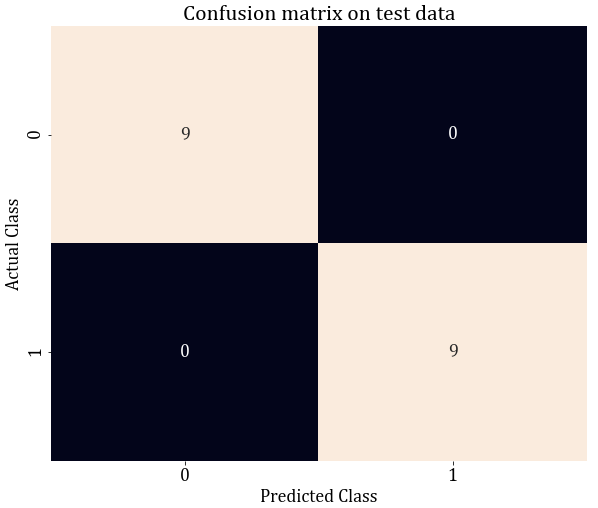
\includegraphics[scale=0.4]{images/1A_ovo_conf13_test.png}
\caption{Confusion matrix for class 1 and 3, train and test data respectively}
\end{figure}

\begin{figure}[H]
\centering
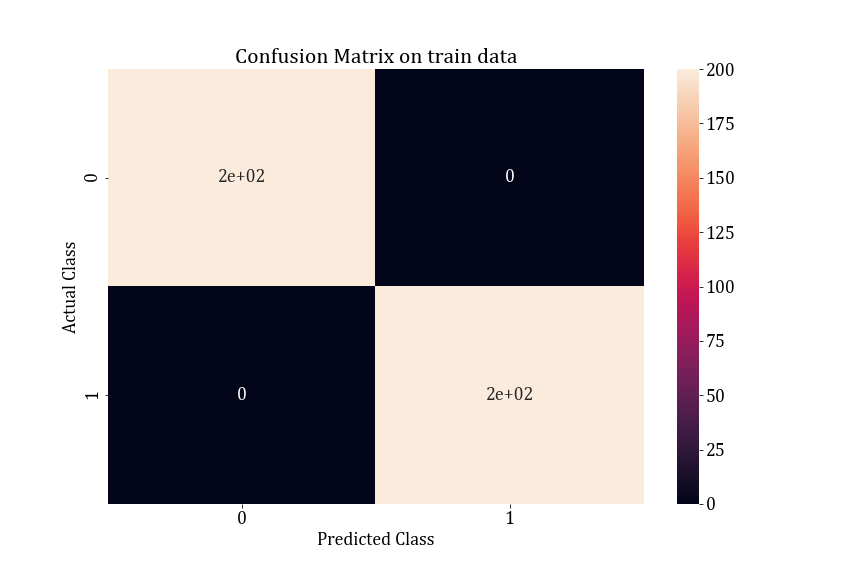
\includegraphics[scale=0.4]{images/1A_ovo_conf23_train.png}
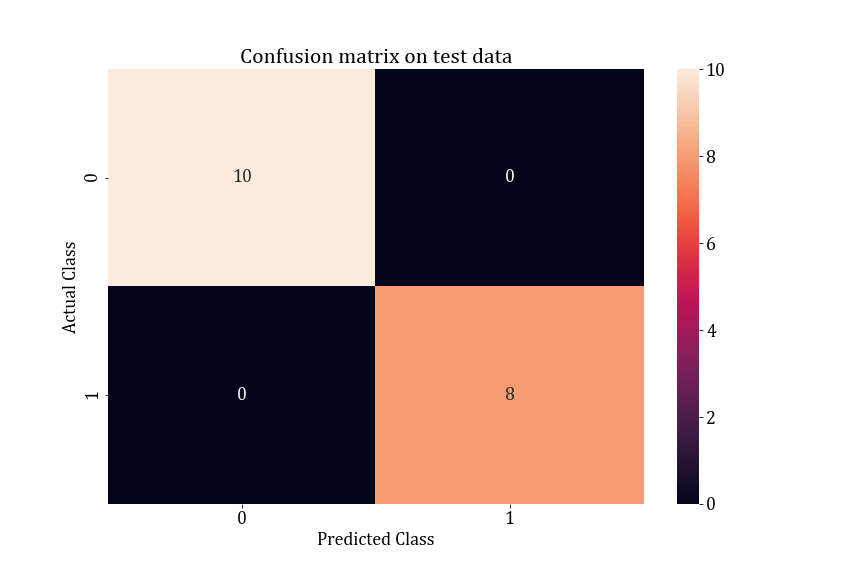
\includegraphics[scale=0.4]{images/1A_ovo_conf23_test.png}
\caption{Confusion matrix for class 2 and 3, train and test data respectively}
\end{figure}
\noi 

\subsubsection{Decision boundaries and Support vectors}
\begin{figure}[H]
    \centering
    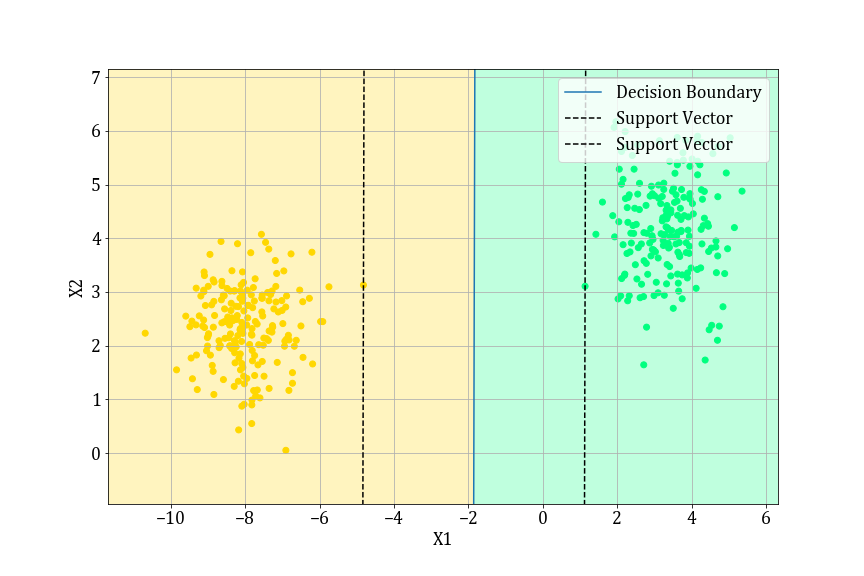
\includegraphics[scale=0.55]{images/1A_ovo_01.png}
    \caption{Decision region for class y=0 and y=1}
\end{figure}

\begin{figure}[H]
    \centering
    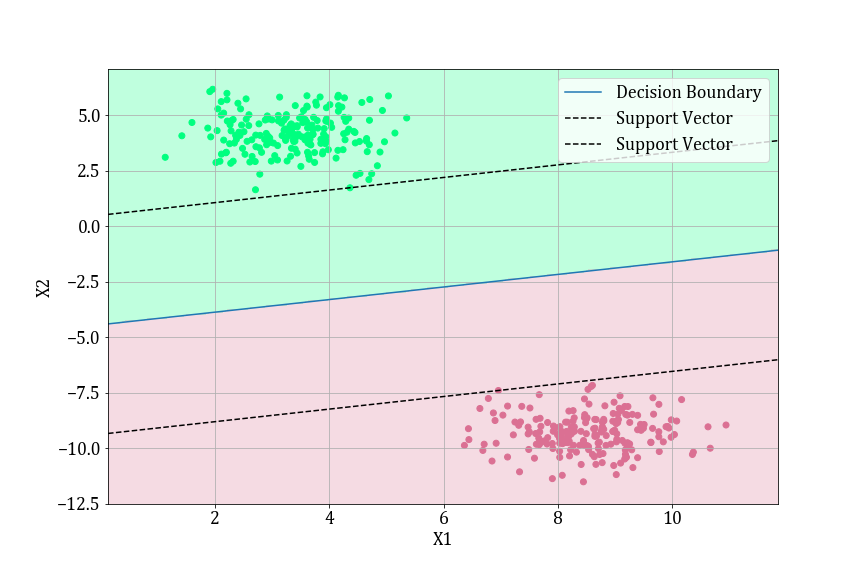
\includegraphics[scale=0.55]{images/1A_ovo_02.png}
    \caption{Decision region for class y=0 and y=2}
\end{figure}

\begin{figure}[H]
    \centering
    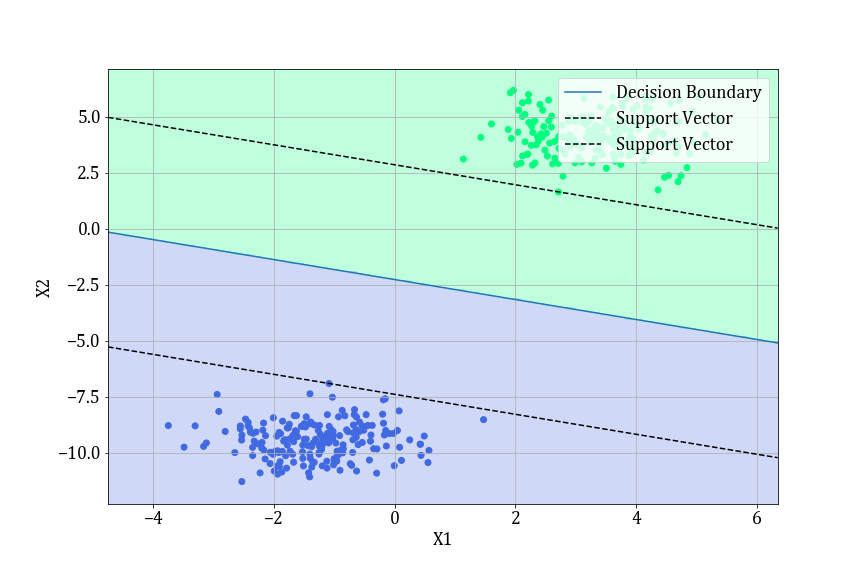
\includegraphics[scale=0.55]{images/1A_ovo_03.png}
    \caption{Decision region for class y=0 and y=3}
\end{figure}

\begin{figure}[H]
    \centering
    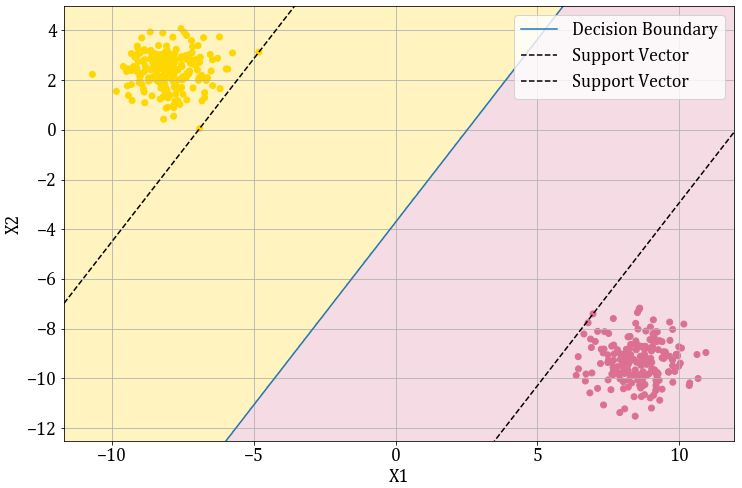
\includegraphics[scale=0.55]{images/1A_ovo_12.png}
    \caption{Decision region for class y=1 and y=2}
\end{figure}

\begin{figure}[H]
    \centering
    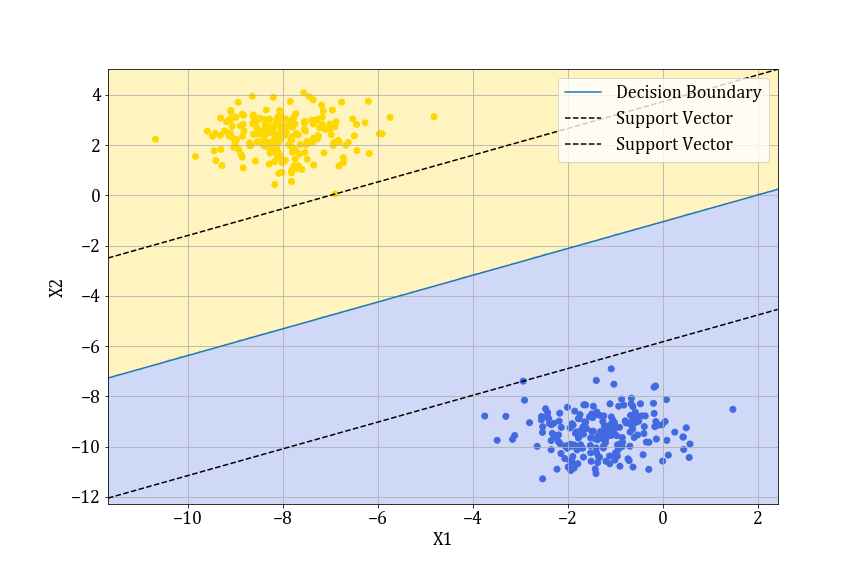
\includegraphics[scale=0.55]{images/1A_ovo_13.png}
    \caption{Decision region for class y=1 and y=3}
\end{figure}

\begin{figure}[H]
    \centering
    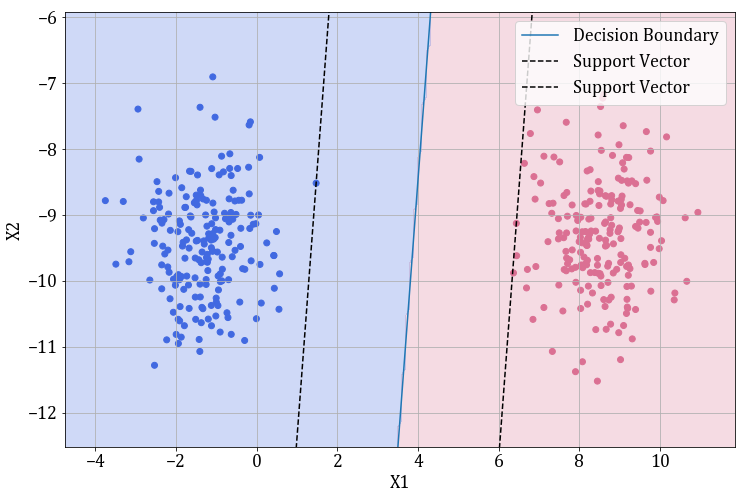
\includegraphics[scale=0.55]{images/1A_ovo_23.png}
    \caption{Decision region for class y=2 and y=3}
\end{figure}

\begin{figure}[H]
    \centering
    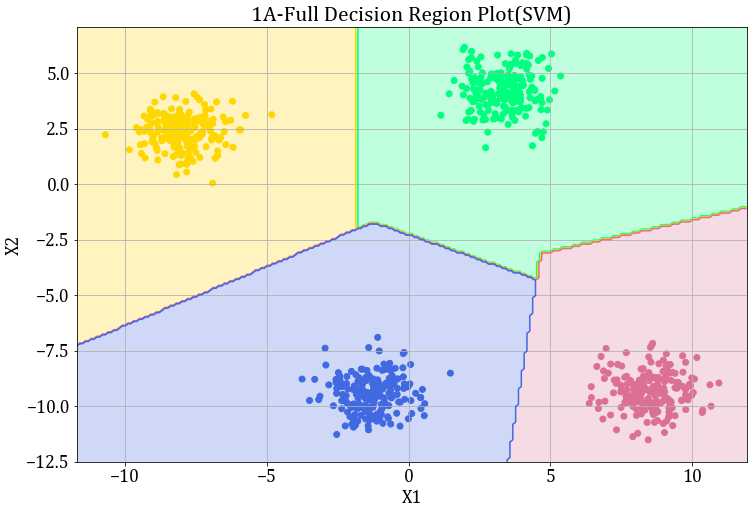
\includegraphics[scale=0.55]{images/1A_SVM_full_decision_plot.png}
    \caption{The effective decision region for dataset 1A}
\end{figure}

\subsubsection{Conclusion}
Observations from one-vs-one decision boundary plots:
\begin{enumerate}
    \item The separating hyper-planes are linear.
    \item The hyper-planes formed by the Support Vectors are parallel to the separating hyper-plane. 
    \item Since no training data points lie between the supporting vector hyper-plane and the separating hyper-plane, it is a hard margin solution. 
\end{enumerate}


\break
%%%%%%%%%%%%%%%%%%%%%%%%%%%%%%%%%%%%%%%%%%%%%%%
%%%%%%%%%%%%%%%%%%%%%%%%%%%%%%%%%%%%%%%%%%%%%%%
\section{Dataset 1B}
This dataset contains data for three classes - 0, 1 and 2. The classes are non-linearly separable and the dimension of the feature space is 2.
%%%%%%%%%%%%%%%%%%%%%%%%%%%%%%%%%%%%%%%%%%%%%%%
%%%%%%%%%%%%%%%%%%%%%%%%%%%%%%%%%%%%%%%%%%%%%%%
\subsection{MLFFNN}
%%%%%%%%%%%%%%%%%%%%%%%%%%%%%%%%%%%%%%%%%%%%%%%%%%
The hyperparameters varied and sweeped for are - \tt{hidden layer size}, \tt{activation function}, \tt{batch size}, \tt{learning rate}, \tt{L2 regularization $\alpha$}. They were varied as follows:
\begin{itemize}
    \itemsep0em
    \item \tt{hidden\_layer\_sizes}: (5,5), (6,6), (7,7), (8,8), (9,9), (10,10)
    \item \tt{activation}: \tt{logistic}, \tt{relu}
    \item \tt{batch\_size}: 50, 100, 200, 
    \item \tt{early\_stopping}: \tt{True}, \tt{False}
    \item \tt{learning\_rate}: \tt{constant}, \tt{adaptive}, \tt{invscaling}
    \item \tt{alpha}: 0.01, 0.001
\end{itemize}

\noi
Hence, a total of 432 parameter combinations were sweeped for and analyzed.

\subsubsection{Classification Accuracies}
The classification accuracies on the training and validation datasets (30\% of the \colortt{dev.csv}) are as follows:
\def\arraystretch{1.25}
\begin{center}
{\small
\begin{tabular}{l l l l l l c c}
\hline
\hline
\textbf{\# Neurons} & \textbf{Activation} & \textbf{Batch Size} & \textbf{Early Stopping} & \textbf{Learning Rate} & \textbf{\alpha} & \textbf{Accuracy} & \textbf{Validation Accuracy} \\
\hline
\hline
(8, 8) & relu & 50 & False & adaptive & 0.01 & 99.33 & 98.41  \\
(8, 8) & relu & 50 & False & constant & 0.001 & 99.33 & 98.41  \\
(8, 8) & relu & 50 & False & invscaling & 0.01 & 99.33 & 98.41  \\
(8, 8) & relu & 50 & False & adaptive & 0.001 & 99.33 & 98.41  \\
(8, 8) & relu & 50 & False & invscaling & 0.001 & 99.33 & 98.41  \\
(8, 8) & relu & 50 & False & constant & 0.01 & 99.33 & 98.41  \\
(10, 10) & relu & 50 & False & adaptive & 0.01 & 99.0 & 98.41  \\
(10, 10) & relu & 50 & False & constant & 0.01 & 99.0 & 98.41  \\
(10, 10) & relu & 50 & False & invscaling & 0.01 & 99.0 & 98.41  \\
(10, 10) & relu & 50 & False & constant & 0.001 & 99.0 & 96.82  \\
\hline
\end{tabular}
\captionof{table}{Best 10 Train and Validation Accuracies obtained after performing a \colortt{GridSearch} on 432 parameter combinations.}
}
\end{center}

\subsubsection{Best Model}
The parameter combination were additionally sorted based on minimum fitting time (least fitting time - first) and the model that gave the best accuracy the fastest (and potentially the most minimal model that best fits the data), was chosen. Hence the best parameter combination chosen is:
\begin{itemize}
    \itemsep0em
    \item hidden\_layer\_sizes: (8, 8)
    \item activation: relu
    \item batch\_size: 50
    \item early\_stopping: False
    \item learning\_rate: adaptive
    \item alpha (L2 regularization): 0.01
\end{itemize}

\noi
The classification accuracy of the best model on the testing data is: \textbf{96.296\%}. The confusion matrices obtained are as follows:
\begin{figure}[H]
    \centering
    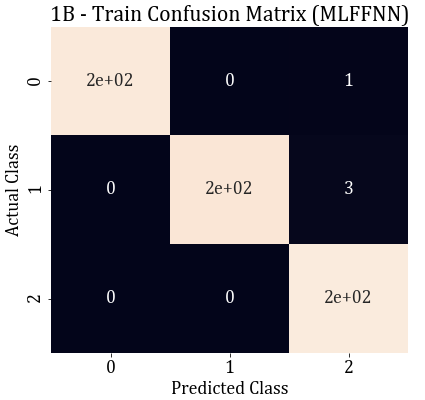
\includegraphics[scale=0.55]{images/1B_MLFFNN_train_confmat.png}
    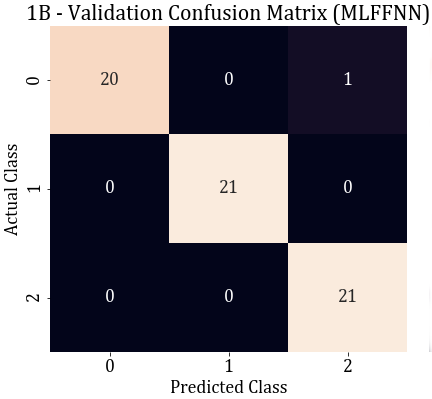
\includegraphics[scale=0.55]{images/1B_MLFFNN_val_confmat.png}
    \caption{Training and Validation confusion matrices obtained for the best parameter combination, on the left and right respectively.}
\end{figure}

\begin{figure}[H]
    \centering
    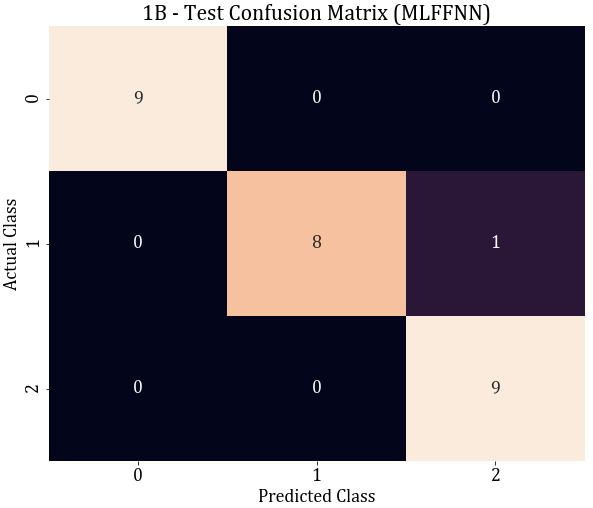
\includegraphics[scale=0.45]{images/1B_MLFFNN_test_confmat.png}
    \caption{Testing confusion matrices obtained for the best parameter combination.}
\end{figure}

\subsubsection{Decision Region}
The decision region plots obtained is as follows:
\begin{figure}[H]
    \centering
    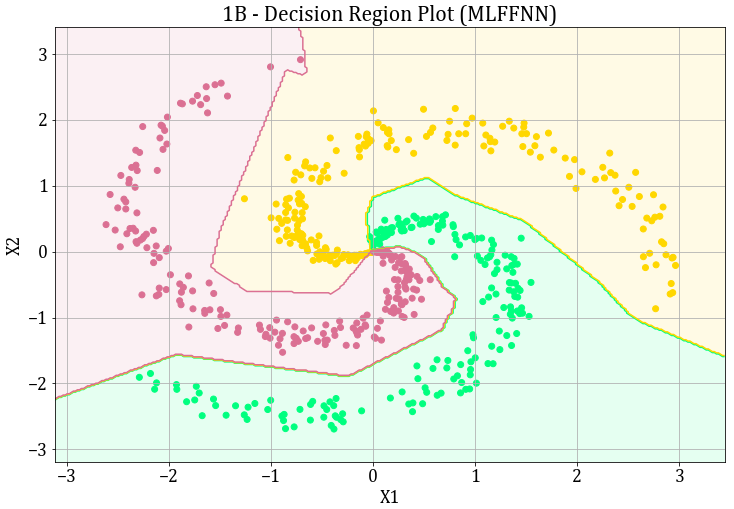
\includegraphics[scale=0.55]{images/1B_MLFFNN_Decision_Plot.png}
    \caption{Decision Region Plot obtained for the best parameter combination.}
\end{figure}

\subsubsection{Surface Plots}
The neuron-wise surface plots obtained for the hidden and output layers is as follows:
\paragraph{Hidden Layer 1, Node 1}
\begin{figure}[H]
    \centering
    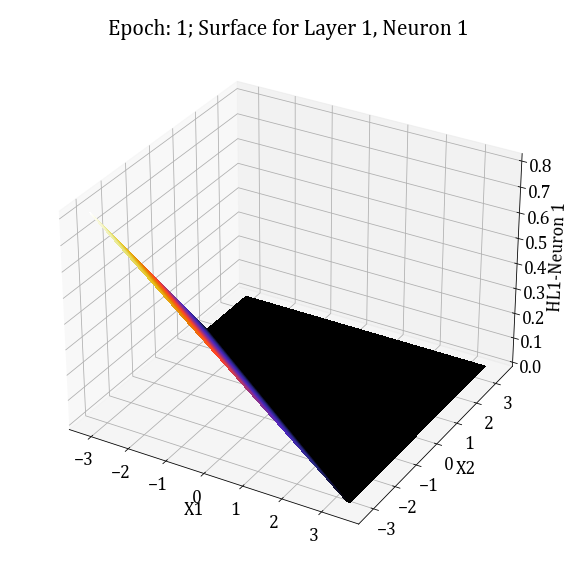
\includegraphics[scale=0.4]{images/1B_MLFFNN_E1_HL1_N1.png}
    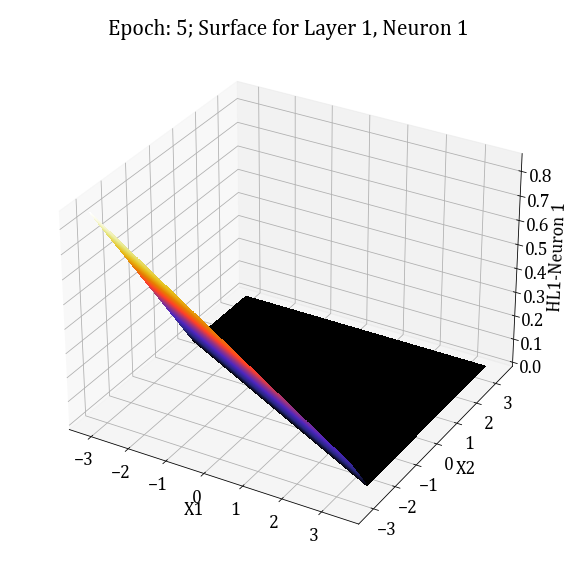
\includegraphics[scale=0.4]{images/1B_MLFFNN_E5_HL1_N1.png}
    \includegraphics[scale=0.4]{images/1B_MLFFNN_E20_HL1_N1.png}
    \includegraphics[scale=0.4]{images/1B_MLFFNN_E100_HL1_N1.png}
    \includegraphics[scale=0.4]{images/1B_MLFFNN_conv_HL1_N1.png}
    \caption{Surface Plots obtained for Hidden Layer 1, Neuron 1, across epochs.}
    \label{HL1N1}
\end{figure}

\paragraph{Hidden Layer 1, Node 2}
\begin{figure}[H]
    \centering
    \includegraphics[scale=0.4]{images/1B_MLFFNN_E1_HL1_N2.png}
    \includegraphics[scale=0.4]{images/1B_MLFFNN_E5_HL1_N2.png}
    \includegraphics[scale=0.4]{images/1B_MLFFNN_E20_HL1_N2.png}
    \includegraphics[scale=0.4]{images/1B_MLFFNN_E100_HL1_N2.png}
    \includegraphics[scale=0.4]{images/1B_MLFFNN_conv_HL1_N2.png}
    \caption{Surface Plots obtained for Hidden Layer 1, Neuron 2, across epochs.}
\end{figure}

\paragraph{Hidden Layer 1, Node 3}
\begin{figure}[H]
    \centering
    \includegraphics[scale=0.4]{images/1B_MLFFNN_E1_HL1_N3.png}
    \includegraphics[scale=0.4]{images/1B_MLFFNN_E5_HL1_N3.png}
    \includegraphics[scale=0.4]{images/1B_MLFFNN_E20_HL1_N3.png}
    \includegraphics[scale=0.4]{images/1B_MLFFNN_E100_HL1_N3.png}
    \includegraphics[scale=0.4]{images/1B_MLFFNN_conv_HL1_N3.png}
    \caption{Surface Plots obtained for Hidden Layer 1, Neuron 3, across epochs.}
\end{figure}

\paragraph{Hidden Layer 1, Node 4}
\begin{figure}[H]
    \centering
    \includegraphics[scale=0.4]{images/1B_MLFFNN_E1_HL1_N4.png}
    \includegraphics[scale=0.4]{images/1B_MLFFNN_E5_HL1_N4.png}
    \includegraphics[scale=0.4]{images/1B_MLFFNN_E20_HL1_N4.png}
    \includegraphics[scale=0.4]{images/1B_MLFFNN_E100_HL1_N4.png}
    \includegraphics[scale=0.4]{images/1B_MLFFNN_conv_HL1_N4.png}
    \caption{Surface Plots obtained for Hidden Layer 1, Neuron 4, across epochs.}
\end{figure}

\paragraph{Hidden Layer 1, Node 5}
\begin{figure}[H]
    \centering
    \includegraphics[scale=0.4]{images/1B_MLFFNN_E1_HL1_N5.png}
    \includegraphics[scale=0.4]{images/1B_MLFFNN_E5_HL1_N5.png}
    \includegraphics[scale=0.4]{images/1B_MLFFNN_E20_HL1_N5.png}
    \includegraphics[scale=0.4]{images/1B_MLFFNN_E100_HL1_N5.png}
    \includegraphics[scale=0.4]{images/1B_MLFFNN_conv_HL1_N5.png}
    \caption{Surface Plots obtained for Hidden Layer 1, Neuron 5, across epochs.}
\end{figure}

\paragraph{Hidden Layer 1, Node 6}
\begin{figure}[H]
    \centering
    \includegraphics[scale=0.4]{images/1B_MLFFNN_E1_HL1_N6.png}
    \includegraphics[scale=0.4]{images/1B_MLFFNN_E5_HL1_N6.png}
    \includegraphics[scale=0.4]{images/1B_MLFFNN_E20_HL1_N6.png}
    \includegraphics[scale=0.4]{images/1B_MLFFNN_E100_HL1_N6.png}
    \includegraphics[scale=0.4]{images/1B_MLFFNN_conv_HL1_N6.png}
    \caption{Surface Plots obtained for Hidden Layer 1, Neuron 6, across epochs.}
\end{figure}

\paragraph{Hidden Layer 1, Node 7}
\begin{figure}[H]
    \centering
    \includegraphics[scale=0.4]{images/1B_MLFFNN_E1_HL1_N7.png}
    \includegraphics[scale=0.4]{images/1B_MLFFNN_E5_HL1_N7.png}
    \includegraphics[scale=0.4]{images/1B_MLFFNN_E20_HL1_N7.png}
    \includegraphics[scale=0.4]{images/1B_MLFFNN_E100_HL1_N7.png}
    \includegraphics[scale=0.4]{images/1B_MLFFNN_conv_HL1_N7.png}
    \caption{Surface Plots obtained for Hidden Layer 1, Neuron 7, across epochs.}
\end{figure}

\paragraph{Hidden Layer 1, Node 8}
\begin{figure}[H]
    \centering
    \includegraphics[scale=0.4]{images/1B_MLFFNN_E1_HL1_N8.png}
    \includegraphics[scale=0.4]{images/1B_MLFFNN_E5_HL1_N8.png}
    \includegraphics[scale=0.4]{images/1B_MLFFNN_E20_HL1_N8.png}
    \includegraphics[scale=0.4]{images/1B_MLFFNN_E100_HL1_N8.png}
    \includegraphics[scale=0.4]{images/1B_MLFFNN_conv_HL1_N8.png}
    \caption{Surface Plots obtained for Hidden Layer 1, Neuron 8, across epochs.}
\end{figure}

\paragraph{Hidden Layer 2, Node 1}
\begin{figure}[H]
    \centering
    \includegraphics[scale=0.4]{images/1B_MLFFNN_E1_HL2_N1.png}
    \includegraphics[scale=0.4]{images/1B_MLFFNN_E5_HL2_N1.png}
    \includegraphics[scale=0.4]{images/1B_MLFFNN_E20_HL2_N1.png}
    \includegraphics[scale=0.4]{images/1B_MLFFNN_E100_HL2_N1.png}
    \includegraphics[scale=0.4]{images/1B_MLFFNN_conv_HL2_N1.png}
    \caption{Surface Plots obtained for Hidden Layer 2, Neuron 1, across epochs.}
\end{figure}

\paragraph{Hidden Layer 2, Node 2}
\begin{figure}[H]
    \centering
    \includegraphics[scale=0.4]{images/1B_MLFFNN_E1_HL2_N2.png}
    \includegraphics[scale=0.4]{images/1B_MLFFNN_E5_HL2_N2.png}
    \includegraphics[scale=0.4]{images/1B_MLFFNN_E20_HL2_N2.png}
    \includegraphics[scale=0.4]{images/1B_MLFFNN_E100_HL2_N2.png}
    \includegraphics[scale=0.4]{images/1B_MLFFNN_conv_HL2_N2.png}
    \caption{Surface Plots obtained for Hidden Layer 2, Neuron 2, across epochs.}
\end{figure}

\paragraph{Hidden Layer 2, Node 3}
\begin{figure}[H]
    \centering
    \includegraphics[scale=0.4]{images/1B_MLFFNN_E1_HL2_N3.png}
    \includegraphics[scale=0.4]{images/1B_MLFFNN_E5_HL2_N3.png}
    \includegraphics[scale=0.4]{images/1B_MLFFNN_E20_HL2_N3.png}
    \includegraphics[scale=0.4]{images/1B_MLFFNN_E100_HL2_N3.png}
    \includegraphics[scale=0.4]{images/1B_MLFFNN_conv_HL2_N3.png}
    \caption{Surface Plots obtained for Hidden Layer 2, Neuron 3, across epochs.}
\end{figure}

\paragraph{Hidden Layer 2, Node 4}
\begin{figure}[H]
    \centering
    \includegraphics[scale=0.4]{images/1B_MLFFNN_E1_HL2_N4.png}
    \includegraphics[scale=0.4]{images/1B_MLFFNN_E5_HL2_N4.png}
    \includegraphics[scale=0.4]{images/1B_MLFFNN_E20_HL2_N4.png}
    \includegraphics[scale=0.4]{images/1B_MLFFNN_E100_HL2_N4.png}
    \includegraphics[scale=0.4]{images/1B_MLFFNN_conv_HL2_N4.png}
    \caption{Surface Plots obtained for Hidden Layer 2, Neuron 4, across epochs.}
\end{figure}

\paragraph{Hidden Layer 2, Node 5}
\begin{figure}[H]
    \centering
    \includegraphics[scale=0.4]{images/1B_MLFFNN_E1_HL2_N5.png}
    \includegraphics[scale=0.4]{images/1B_MLFFNN_E5_HL2_N5.png}
    \includegraphics[scale=0.4]{images/1B_MLFFNN_E20_HL2_N5.png}
    \includegraphics[scale=0.4]{images/1B_MLFFNN_E100_HL2_N5.png}
    \includegraphics[scale=0.4]{images/1B_MLFFNN_conv_HL2_N5.png}
    \caption{Surface Plots obtained for Hidden Layer 2, Neuron 5, across epochs.}
\end{figure}

\paragraph{Hidden Layer 2, Node 6}
\begin{figure}[H]
    \centering
    \includegraphics[scale=0.4]{images/1B_MLFFNN_E1_HL2_N6.png}
    \includegraphics[scale=0.4]{images/1B_MLFFNN_E5_HL2_N6.png}
    \includegraphics[scale=0.4]{images/1B_MLFFNN_E20_HL2_N6.png}
    \includegraphics[scale=0.4]{images/1B_MLFFNN_E100_HL2_N6.png}
    \includegraphics[scale=0.4]{images/1B_MLFFNN_conv_HL2_N6.png}
    \caption{Surface Plots obtained for Hidden Layer 2, Neuron 6, across epochs.}
\end{figure}

\paragraph{Hidden Layer 2, Node 7}
\begin{figure}[H]
    \centering
    \includegraphics[scale=0.4]{images/1B_MLFFNN_E1_HL2_N7.png}
    \includegraphics[scale=0.4]{images/1B_MLFFNN_E5_HL2_N7.png}
    \includegraphics[scale=0.4]{images/1B_MLFFNN_E20_HL2_N7.png}
    \includegraphics[scale=0.4]{images/1B_MLFFNN_E100_HL2_N7.png}
    \includegraphics[scale=0.4]{images/1B_MLFFNN_conv_HL2_N7.png}
    \caption{Surface Plots obtained for Hidden Layer 2, Neuron 7, across epochs.}
\end{figure}

\paragraph{Hidden Layer 2, Node 8}
\begin{figure}[H]
    \centering
    \includegraphics[scale=0.4]{images/1B_MLFFNN_E1_HL2_N8.png}
    \includegraphics[scale=0.4]{images/1B_MLFFNN_E5_HL2_N8.png}
    \includegraphics[scale=0.4]{images/1B_MLFFNN_E20_HL2_N8.png}
    \includegraphics[scale=0.4]{images/1B_MLFFNN_E100_HL2_N8.png}
    \includegraphics[scale=0.4]{images/1B_MLFFNN_conv_HL2_N8.png}
    \caption{Surface Plots obtained for Hidden Layer 2, Neuron 8, across epochs.}
\end{figure}

\paragraph{Output Layer, Node 1}
\begin{figure}[H]
    \centering
    \includegraphics[scale=0.4]{images/1B_MLFFNN_E1_OP_N1.png}
    \includegraphics[scale=0.4]{images/1B_MLFFNN_E5_OP_N1.png}
    \includegraphics[scale=0.4]{images/1B_MLFFNN_E20_OP_N1.png}
    \includegraphics[scale=0.4]{images/1B_MLFFNN_E100_OP_N1.png}
    \includegraphics[scale=0.4]{images/1B_MLFFNN_conv_OP_N1.png}
    \caption{Surface Plots obtained for Output Layer, Neuron 1, across epochs.}
\end{figure}

\paragraph{Output Layer, Node 2}
\begin{figure}[H]
    \centering
    \includegraphics[scale=0.4]{images/1B_MLFFNN_E1_OP_N2.png}
    \includegraphics[scale=0.4]{images/1B_MLFFNN_E5_OP_N2.png}
    \includegraphics[scale=0.4]{images/1B_MLFFNN_E20_OP_N2.png}
    \includegraphics[scale=0.4]{images/1B_MLFFNN_E100_OP_N2.png}
    \includegraphics[scale=0.4]{images/1B_MLFFNN_conv_OP_N2.png}
    \caption{Surface Plots obtained for Output Layer, Neuron 2, across epochs.}
\end{figure}

\paragraph{Output Layer, Node 3}
\begin{figure}[H]
    \centering
    \includegraphics[scale=0.4]{images/1B_MLFFNN_E1_OP_N3.png}
    \includegraphics[scale=0.4]{images/1B_MLFFNN_E5_OP_N3.png}
    \includegraphics[scale=0.4]{images/1B_MLFFNN_E20_OP_N3.png}
    \includegraphics[scale=0.4]{images/1B_MLFFNN_E100_OP_N3.png}
    \includegraphics[scale=0.4]{images/1B_MLFFNN_conv_OP_N3.png}
    \caption{Surface Plots obtained for Output Layer, Neuron 3, across epochs.}
    \label{OPN3}
\end{figure}

\noi
From \autoref{HL1N1}-\autoref{OPN3}, we observe the following:
\begin{itemize}
    \itemsep0em 
    \item First hidden layer surface plot is non-linear (activation function is \colortt{ReLU}). However, the surfaces obtained are hyperplanes.
    \item Responses from the second layer is highly non-linear and the surfaces are very comples.
    \item The surface plot of the output neurons shows the selection cum localization of different classes in the latent space.
\end{itemize}

%%%%%%%%%%%%%%%%%%%%%%%%%%%%%%%%%%%%%%%%%%%%%%%
\subsection{Non-Linear SVM}

The module \tt{sklearn.svm.SVC()} as described in section \ref{subsubsection:svm module} is used to build non-linear classifiers for dataset 1B with the parameter ``decision\_function\_shape'' set to ``ovr''. The module can carry out multi-class classification hence individual pair-wise models need not be built.  
\noi
The kernels used for classification are:
\begin{itemize}
    \itemsep0em
    \item Polynomial Kernel-\\
    It is defined as $(\gamma<x,x'>+r)^d$. Where $\gamma$, r and d are the hyper-parameters.
    \item Gaussian Kernel or the Radial Basis function kernel-\\
    It is defined as $exp(-\gamma||x-x'||^2)$. Where $\gamma$ is the hyper-parameter.
\end{itemize}

\subsubsection{Polynomial Kernel}
While using this kernel, a number of hyper-parameters need to be set: 
\begin{itemize}
    \itemsep0em
    \item misclassification penalty term, \tt{C}.
    \item Coefficient of the polynomials, $\gamma$.
    \item Constant term in the kernel, \tt{r}.
    \item Degree of the polynomial, \tt{d}.
\end{itemize}

\noi
Due to a large number of possible combinations of the above hyper-parameters, we use the function \tt{GridSearchCV} from \tt{sklearn.model\_selection} to search for the optimal combination of hyper-parameters.

\subsubsection{Optimal hyper-parameters and accuracy: Polynomial Kernel}

The following values of hyper-parameters are tried resulting in $4*6*2*4=192$ different models.  
\begin{itemize}
    \itemsep0em
    \item \tt{C}: [1,10,100,1000]
    \item \tt{degree}: [1,2,3,4,5,6]
    \item \tt{coef0}: [10,100]
    \item $\gamma$: [1,0.1,0.01,``auto'']
\end{itemize}

\noi
The function \tt{GridSearchCV} returns the validation and train accuracy for all the models in the form of a numpy array. Accuracy table for the 10 models with the highest validation accuracy is: 
\def\arraystretch{1.25}
\begin{longtable}{l l l l l l}
\hline
\hline
\textbf{C} & \textbf{degree} & \textbf{gamma} & \textbf{Coef0} & \textbf{Train Accuracy} & \textbf{Validation Accuracy}\\
\hline
\hline
1000 & 5 & 0.1 & 100 & 0.983 & 1.00 \\
10 & 4 & 0.1 & 10 & 0.993 & 0.981 \\
1 & 5 & 0.1 & 100 & 0.986 & 0.976  \\
1 & 3 & 1 & 10 & 0.995 & 0.977 \\
100 & 5 & 0.1 & 100 & 0.981 & 0.977 \\
10 & 5 & 0.1 & 100 & 0.981 & 0.977 \\
1 & 3 & "auto" & 100 & 0.980 & 0.975 \\
1000 & 3 & 0.1 & 10 & 0.995 & 0.975 \\
100 & 3 & 0.1 & 10 & 0.980 & 0.975 \\
100 & 5 & 0.01 & 10 & 0.985 & 0.975 \\

\hline
\caption{Accuracy table for dataset 1B - SVM classifier with polynomial kernel}
\end{longtable}


\noi
Since the validation accuracy is highest for [C:1000,degree:5,gamma:0.1,Coef0:100], those hyper-parameters are used to predict the class labels for the test dataset, obtaining an accuracy of \textbf{1.00}. Those hyper-parameters are further used to obtain the confusion matrices and to plot the decision boundaries. 

\subsubsection{Confusion matrices for Train and Test data: Polynomial Kernel}

\begin{figure}[H]
    \centering
    \includegraphics[scale=0.4]{images/1B_SVM_poly_train_confmat.png}
    \includegraphics[scale=0.4]{images/1B_SVM_poly_Test_confmat.png}
    \caption{Confusion matrix for Train and Test data respectively}
\end{figure}

\subsubsection{Decision Region: Polynomial Kernel}

\begin{figure}[H]
    \centering
    \includegraphics[scale=0.5]{images/1B_SVM_poly_decision_plot.png}
    \caption{Decision Region Plot for dataset 1B}
    \label{myfig:poly_db}
\end{figure}

\subsubsection{SVM with gaussian kernel}\label{section:gaussian}

While using this kernel, the number of hyper-parameters to be set are comparatively less.
\begin{itemize}
    \item misclassification penalty term, C; Varied over [0.1,1,10,100,1000]
    \item Coefficient $\gamma$, varied over: [1,0.01,0.001,0.0001]
\end{itemize}

\subsubsection{Optimal hyper-parameters and accuracy: Gaussian Kernel}

Corresponding to different combinations of the above hyper-parameter values, 20 different models are trained. The training accuracy and cross-validation accuracy are obtained as follows:  
\noi
\def\arraystretch{1.25}
\begin{center}
{\small
\begin{longtable}{l l l l l l l l}
\hline
\hline
\textbf{gamma} & \textbf{C} & \textbf{Train Accuracy}  & \textbf{Val. Accuracy} & \textbf{gamma} & \textbf{C} & \textbf{Train Accuracy}  & \textbf{Val. Accuracy}\\
\hline
\hline
1.00 & 1.0 & 99.16 & 100 & 0.001 & 0.1 & 51.67 & 53.96 \\
1.00 & 0.1 & 99.16 & 98.41  & 0.001 & 1.0 & 51.50 & 53.96 \\
1.00 & 10.0 & 99.66 & 98.41  & 0.001 & 10.0 & 51.50 & 60.31 \\
1.00 & 100.0 & 99.66 & 98.41  & 0.001 & 100.0 & 54.17 & 61.90 \\
1.00 & 1000.0 & 99.83 & 96.82  & 0.001 & 1000.0 & 84.67 & 80.95\\
0.01 & 0.1 & 51.16 & 55.56  & 0.0001 & 0.1 & 51.50 & 53.97 \\
0.01 & 1.0 & 53.17 & 61.90  & 0.0001 & 1.0 & 51.50 & 53.97 \\
0.01 & 10.0 & 84.83 & 80.95  & 0.0001 & 10.0 & 51.17 & 53.97 \\
0.01 & 100.0 & 86.83 & 80.95  & 0.0001 & 100.0 & 51.50 & 60.32 \\
0.01 & 1000.0 & 92.16 & 87.30  & 0.0001 & 1000.0 & 50.83 & 60.32 \\
\hline
\end{longtable}
\setcounter{table}{2}
\captionof{table}{Accuracy table for data set 1B: SVM with Gaussian Kernel}
}
\end{center}

\noi
The validation accuracy is highest for [C:1.0, gamma:1.0]. Hence those hyper-parameters are used for further calculations. Accuracy on test data with those hyper-parameters is obtained to be \textbf{100\%}. 

\subsubsection{Confusion matrices for Train and Test data: Gaussian Kernel}

\begin{figure}[H]
    \centering
    \includegraphics[scale=0.4]{images/1B_SVM_gauss_train_confmat.png}
    \includegraphics[scale=0.4]{images/1B_SVM_gauss_Test_confmat.png}
    \caption{Confusion Matrix for Train and Test data respectively}
\end{figure}

\subsubsection{Decision Region plot: Gaussian Kernel}

\begin{figure}[H]
    \centering
    \includegraphics[scale=0.5]{images/1B_SVM_gauss_decision_plot.png}
    \caption{Decision region plot for dataset 1B: SVM with Gaussian Kernel}
    \label{myfig:gauss_db}
\end{figure}

\noi
Observations:
\begin{enumerate}
\item The distinguishing feature between \autoref{myfig:gauss_db} and \autoref{myfig:poly_db} is the behavior at the edges. Also, the decision boundary obtained using polynomial kernel has a discontinuity in the region $x_1 \in (-0.5,0.5)$ and $x_2 \in (3,4)$
\item The distribution of support vectors is very distinct. In polynomial kernel, the support vectors are majorly near the center. While in the gaussian kernel, the support vectors are more uniformly distributed.
\end{enumerate}
%%%%%%%%%%%%%%%%%%%%%%%%%%%%%%%%%%%%%%%%%%%%%%%
\break
%%%%%%%%%%%%%%%%%%%%%%%%%%%%%%%%%%%%%%%%%%%%%%%
\section{Dataset 2A}
%%%%%%%%%%%%%%%%%%%%%%%%%%%%%%%%%%%%%%%%%%%%%%%
%%%%%%%%%%%%%%%%%%%%%%%%%%%%%%%%%%%%%%%%%%%%%%%
This dataset contains data for five classes. The classes assigned for our team are: \tt{coast}, \tt{highway}, \tt{mountain}, \tt{opencountry} and \tt{tallbuilding}. These classes were assigned the class label 0, 1, 2, 3 and 4 respectively. The classes are non-linearly separable and the dimension of the feature space is 24.

%%%%%%%%%%%%%%%%%%%%%%%%%%%%%%%%%%%%%%%%%%%%%%%
\subsection{MLFFNN}
%%%%%%%%%%%%%%%%%%%%%%%%%%%%%%%%%%%%%%%%%%%%%%%
An initial parameter search by varying the parameters of the MLFFNN alone was done. However, the accuracy of the model couldn't be improved. In order to increase the accuracy of the model, PCA was used to reduce the dimensionality of the model.\\

\noi
The hyperparameters varied and sweeped for are - \tt{PCA \# components} \tt{MLFFNN hidden layer size}, \tt{MLFFNN batch size}, \tt{MLFFNN learning rate} and \tt{MLFFNN L2 regularization $\alpha$}. They were varied as follows:
\begin{itemize}
    \itemsep0em
    \item \tt{pca\_\_n\_components}: \tt{list(range(1,25))}
    \item \tt{mlp\_\_hidden\_layer\_sizes}: (10,10), (25,25), (50,50), (75,75)
    \item \tt{mlp\_\_batch\_size}: 50, 100, 200
    \item \tt{mlp\_\_alpha}: 0.01, 0.001
    \item \tt{mlp\_\_learning\_rate}: \tt{constant}, \tt{adaptive}, \tt{invscaling}
\end{itemize}

\noi
Hence, a total of 1728 parameter combinations were sweeped for and analyzed.


\subsubsection{Classification Accuracies}
The classification accuracies on the training and validation datasets (30\% of the \colortt{dev.csv}) are as follows:
\def\arraystretch{1.25}
\begin{center}
{\small
\begin{tabular}{l l l l l l c c}
\hline
\hline
\textbf{\# Components} & \textbf{\# Neurons} & \textbf{Learning Rate} & \textbf{Batch Size} & \textbf{\alpha} & \textbf{Accuracy} & \textbf{Validation Accuracy} \\
\hline
\hline
16 & (50, 50) & invscaling & auto & 0.001 & 79.02 & 52.23 \\
16 & (50, 50) & adaptive & auto & 0.001 & 79.02 & 52.23 \\
16 & (50, 50) & constant & auto & 0.001 & 79.02 & 52.23 \\
20 & (50, 50) & constant & auto & 0.010 & 82.93 & 51.82 \\
20 & (50, 50) & adaptive & auto & 0.010 & 82.93 & 51.82 \\
20 & (50, 50) & invscaling & auto & 0.010 & 82.93 & 51.82 \\
8 & (75, 75) & invscaling & 100 & 0.010 & 75.45 & 51.82 \\
19 & (25, 25) & adaptive & auto & 0.001 & 68.05 & 51.42 \\
19 & (25, 25) & constant & auto & 0.001 & 68.05 & 51.42 \\
19 & (25, 25) & invscaling & auto & 0.001 & 68.05 & 51.42 \\
\hline
\end{tabular}
\captionof{table}{Best 10 Train and Validation Accuracies obtained after performing a \colortt{GridSearch} on 1728 parameter combinations.}
}
\end{center}

\subsubsection{Best Model}
The parameter combination were additionally sorted based on minimum fitting time (least fitting time - first) and the model that gave the best accuracy the fastest (and potentially the most minimal model that best fits the data), was chosen. Hence the best parameter combination chosen is:
\begin{itemize}
    \itemsep0em
    \item n\_components: 16
    \item hidden\_layer\_sizes: (50, 50)
    \item batch\_size: 200
    \item alpha: 0.001
    \item learning\_rate: invscaling
\end{itemize}

\noi
The classification accuracy of the best model on the testing data is: \textbf{49.06\%}. \\

\noi
The confusion matrices obtained are as follows:
\begin{figure}[H]
    \centering
    \includegraphics[scale=0.4]{images/2A_MLFFNN_train_confmat.png}
    \includegraphics[scale=0.4]{images/2A_MLFFNN_val_confmat.png}
    \caption{Training and Validation confusion matrices obtained for the best parameter combination, on the left and right respectively.}
\end{figure}

\begin{figure}[H]
    \centering
    \includegraphics[scale=0.45]{images/2A_MLFFNN_test_confmat.png}
    \caption{Testing confusion matrices obtained for the best parameter combination.}
\end{figure}


\subsection{Gaussian-kernel SVM}

Similar to the section \ref{section:gaussian}, an svm classifier with Gaussian kernel is built. However, the accuracy obtained with varying C and gamma is quite low, therefore other parameters of the svm.SVC()  function (like tolerance, class\_weight etc) are also altered to check for better solutions. We find that altering those extra parameters do not affect the accuracy and so are not listed in the accuracy table.

\subsubsection{Optimal Hyper-parameter and accuracy}

Approximately 1500 models were trained, performance of few of those models is as listed below (in order of decreasing validation accuracy)

\def\arraystretch{1.25}
\begin{center}
\begin{longtable}{l l l l}
\hline
\hline
\textbf{C} & \textbf{Gamma} & \textbf{Train Accuracy} & \textbf{Validation Accuracy}\\
\hline
\hline
10 & 1 & 0.80 & 0.51  \\
1000 & 0.1 & 0.79 & 0.51  \\
1000 & "scale & 1.00 & 0.49 \\
100 & "auto" & 0.59 & 0.45 \\
100 & 0.01 & 0.55 & 0.43 \\
0.1 & "scale" & 0.51 & 0.41 \\
1 & 0.1 & 0.47 & 0.39 \\ 
\hline
\end{longtable}
\setcounter{table}{3}
\captionof{table}{Accuracy table for data set 2a- SVM with gaussian kernel}
\end{center}

The best hyper-parameter settings are: [c=1.0, gamma=1.0]. Test accuracy with those hyper-parameters is obtained to be \textbf{0.547}

\subsubsection{Confusion matrix: Gaussian kernel}

\begin{figure}[H]
    \centering
    \includegraphics[scale=0.4]{images/2A_SVM_gauss_train_confmat.png}
    \includegraphics[scale=0.4]{images/2A_SVM_gauss_Test_confmat.png}
    \caption{Confusion matrix for Train and Test data respectively, dataset 2a}
\end{figure}

\subsubsection{Conclusion}
The accuracy obtained with SVM classifier with a gaussian kernel is low. However, it does not improve on carrying out dimension reduction or scaling of the feature vectors. Moreover, the covariance between the feature vectors is very low,below 0.2 for majority while the covariance is maximum at 0.64 for few pairs of feature vectors. 


\end{document}
